\documentclass[spanish,xcolor=pdftex,dvipsnames,table,mathserif]{scrartcl}
%\usepackage[T1]{fontenc}
%\usepackage[utf8]{inputenc}
\usepackage{fontspec,hpprime}
\setsansfont{CMU Sans Serif}%{Arial}
\setmainfont{CMU Serif}%{Times New Roman}
\setmonofont{CMU Typewriter Text}%{Consolas}
\usepackage{amsmath}
%\usepackage{avant}
\usepackage{calc}
\usepackage{bm}
\usepackage{ifthen}
\usepackage[letterpaper]{geometry}
\geometry{verbose,tmargin=2cm,bmargin=2cm,lmargin=2cm,rmargin=2cm,headheight=1cm,headsep=0.3cm,footskip=1cm}
\usepackage{fancyhdr}
\pagestyle{fancy}
\usepackage{graphicx}
\usepackage[spanish]{babel}
\usepackage{mathabx}
\usepackage{array}
\usepackage{multirow}
\usepackage{lastpage}
\usepackage{pdflscape}
\usepackage{dingbat}
\usepackage{amsmath} 
\usepackage{float}
\usepackage{booktabs}
%\aboverulesep=0ex
%\belowrulesep=0ex
\usepackage{longtable}
\usepackage{rotating}
\usepackage[labelsep=period]{caption}
\usepackage{subcaption}
\usepackage[framemethod=TikZ]{mdframed}
\usepackage{varwidth}
%\usepackage{MnSymbol}
%\usepackage{svg}
\usepackage[pdftex,
pdfauthor={Edwin Córdoba},
pdftitle={SecHP},
pdfsubject={Manual de Usuario},
pdfkeywords={Hp Prime SecHP, sección perfiles centroides momentos inercia},
pdfproducer={LaTeX},
pdfcreator={pdflatex}]{hyperref}
\hypersetup{pdfencoding=auto,colorlinks=true,allcolors=black}
\usepackage{tikz}
\usetikzlibrary{calc,snakes}
\addto\shorthandsspanish{\spanishdeactivate{~<>}}
\usetikzlibrary{arrows,backgrounds,mindmap,shapes,patterns,intersections,decorations.pathmorphing,positioning,fit,petri,circuits.logic.US,circuits.logic.IEC,shapes.gates.logic.IEC}
\title{SecHP V 2.1\\HP Prime}
\subtitle{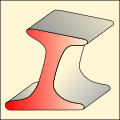
\includegraphics{./imagenes/icon} }
\author{\normalfont \sffamily ©2000-2020\\Edwin Córdoba\\edwin.cordoba@gmail.com}
\addto\captionsspanish{
	\renewcommand{\tablename}{Tabla}
	\renewcommand{\listtablename}{Lista de Tablas}
	\renewcommand{\listfigurename}{Lista de Figuras}
}
\setlength{\parindent}{0pt}
\newenvironment{car}[2][]{%
	%\refstepcounter{car}%
	\ifstrempty{#1}%
	{\mdfsetup{%
			frametitle={%
				\tikz[baseline=(current bounding box.east),outer sep=0pt]
				\node[anchor=east,rectangle,fill=black!20]
				{};}}
	}%
	{\mdfsetup{%
			frametitle={%
				\tikz[baseline=(current bounding box.east),outer sep=0pt]
				\node[anchor=east,rectangle,fill=black!20,execute at begin node={\begin{varwidth}{16.5cm}},
					execute at end node={\end{varwidth}}]
				{#1};}}%
	}%
	\mdfsetup{innertopmargin=10pt,linecolor=black!20,%
		linewidth=2pt,topline=true,%
		frametitleaboveskip=\dimexpr-\ht\strutbox\relax
	}
	%\addcontentsline{c}{car}{ \protect\numberline{\thecar} #1}\par
	\begin{mdframed}[]\relax% 
		%\itshape
		\label{#2}
	}{
\end{mdframed}}

\begin{document}

\thispagestyle{empty}
\maketitle
\thispagestyle{empty}
\begin{abstract}
Este documento corresponde al manual del usuario de la aplicación \verb|SecHP|, desarrollada para las calculadoras gráficas HP Prime. \verb|SecHP| es una aplicación para el cálculo de centro de masa y momentos de inercias de figuras geométricas compuestas.

\noindent La primera versión del programa \verb|SecHP| para la calculadoras gráficas HP Prime fue la versión 2.0, pero su código está basado de los programas \verb|sección| y \verb|SECC++|(programado con las bibliotecas de HPGCC3) desarrollado en las plataformas de las series \verb|HP48| y \verb|HP49|.

\noindent Este programa es gratuito y se proporciona ``COMO ES'', por lo que no se puede ofrecer ninguna garantía de que esté libre de errores, ha sido probado extensamente, pero usted como usuario asume todos los riesgos al utilizarlo.

\end{abstract}
\newpage
\thispagestyle{empty}
\renewcommand{\contentsname}{TABLA DE CONTENIDO}
\tableofcontents
\newpage
\thispagestyle{empty}
\listoftables
\newpage
\thispagestyle{empty}
\listoffigures
\newpage
\setcounter{page}{1}
\section{Cambios.}
\begin{description}
	\item[Nuevo en la versión 2.1] ~
	\begin{itemize}
		\item Se agregó el comando PER(n), que devuelve las propiedades de un perfil seleccionado según el índice de  unidades n.
		\item Se agregó el comando VER, que retorna la versión actual del programa.
		\item En la presentación tabla de resultados, se normalizó para que todas las áreas negativas muestren todos los valores negativos.
	\end{itemize}
\end{description}
\section{Descripción del programa.}
\begin{figure}[H]
	\centering
	\caption{Ejemplo de funcionamiento de la aplicación.}
	\label{fig:ejemplo}
	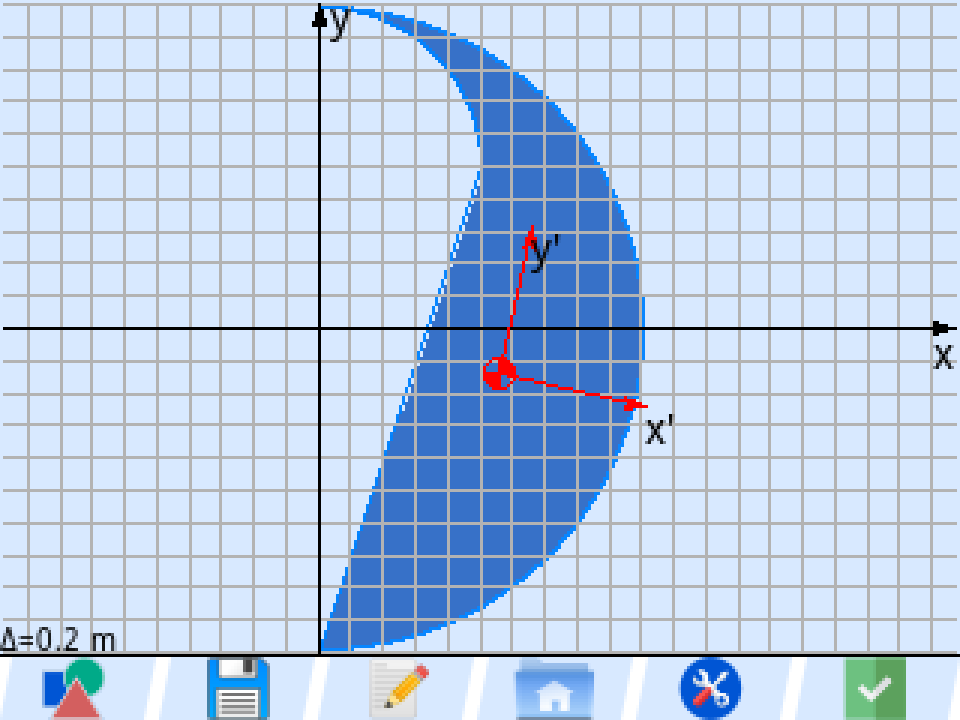
\includegraphics[width=0.5\linewidth]{imagenes/ejemplo}
\end{figure}

Este es un programa para el cálculo de las principales propiedades de una sección conformadas por figuras geométricas compuestas, en la Figura \ref{fig:ejemplo} se muestra un ejemplo de funcionamiento de la aplicación. El programa permite el ingreso de polígonos, círculos, sectores circulares, rectángulos y perfiles de vigas. También permite guardar los datos en un archivo, y por defecto usa el archivo llamado \verb|datos|, para guardar información de la última figura trabajada. Si la calculadora tiene configurado el idioma español, todos los mensajes mostrados serán en español, en caso contrario todos los mensajes serán mostrados en inglés.
\section{Instalación del programa.}
\begin{enumerate}
	\item Descargue e instale el Kit de Conectividad HP (HP Prime Connectivity Kit).
	\item Ejecute el programa Kit de Conectividad HP.
	\item Conecte la calculadora al puerto USB.
	\item Arrastre la carpeta \verb|SecHP.hpappdir| y la suelta en Biblioteca de Aplicaciones (Application Library) como se muestra en la Figura \ref{fig:instalacion}.
	\item La aplicación SecHP deberá aparecer en la biblioteca de aplicaciones.
\end{enumerate}
\begin{figure}[H]
	\centering
	\caption{Instalación de la aplicación SecHP.}
	\label{fig:instalacion}
	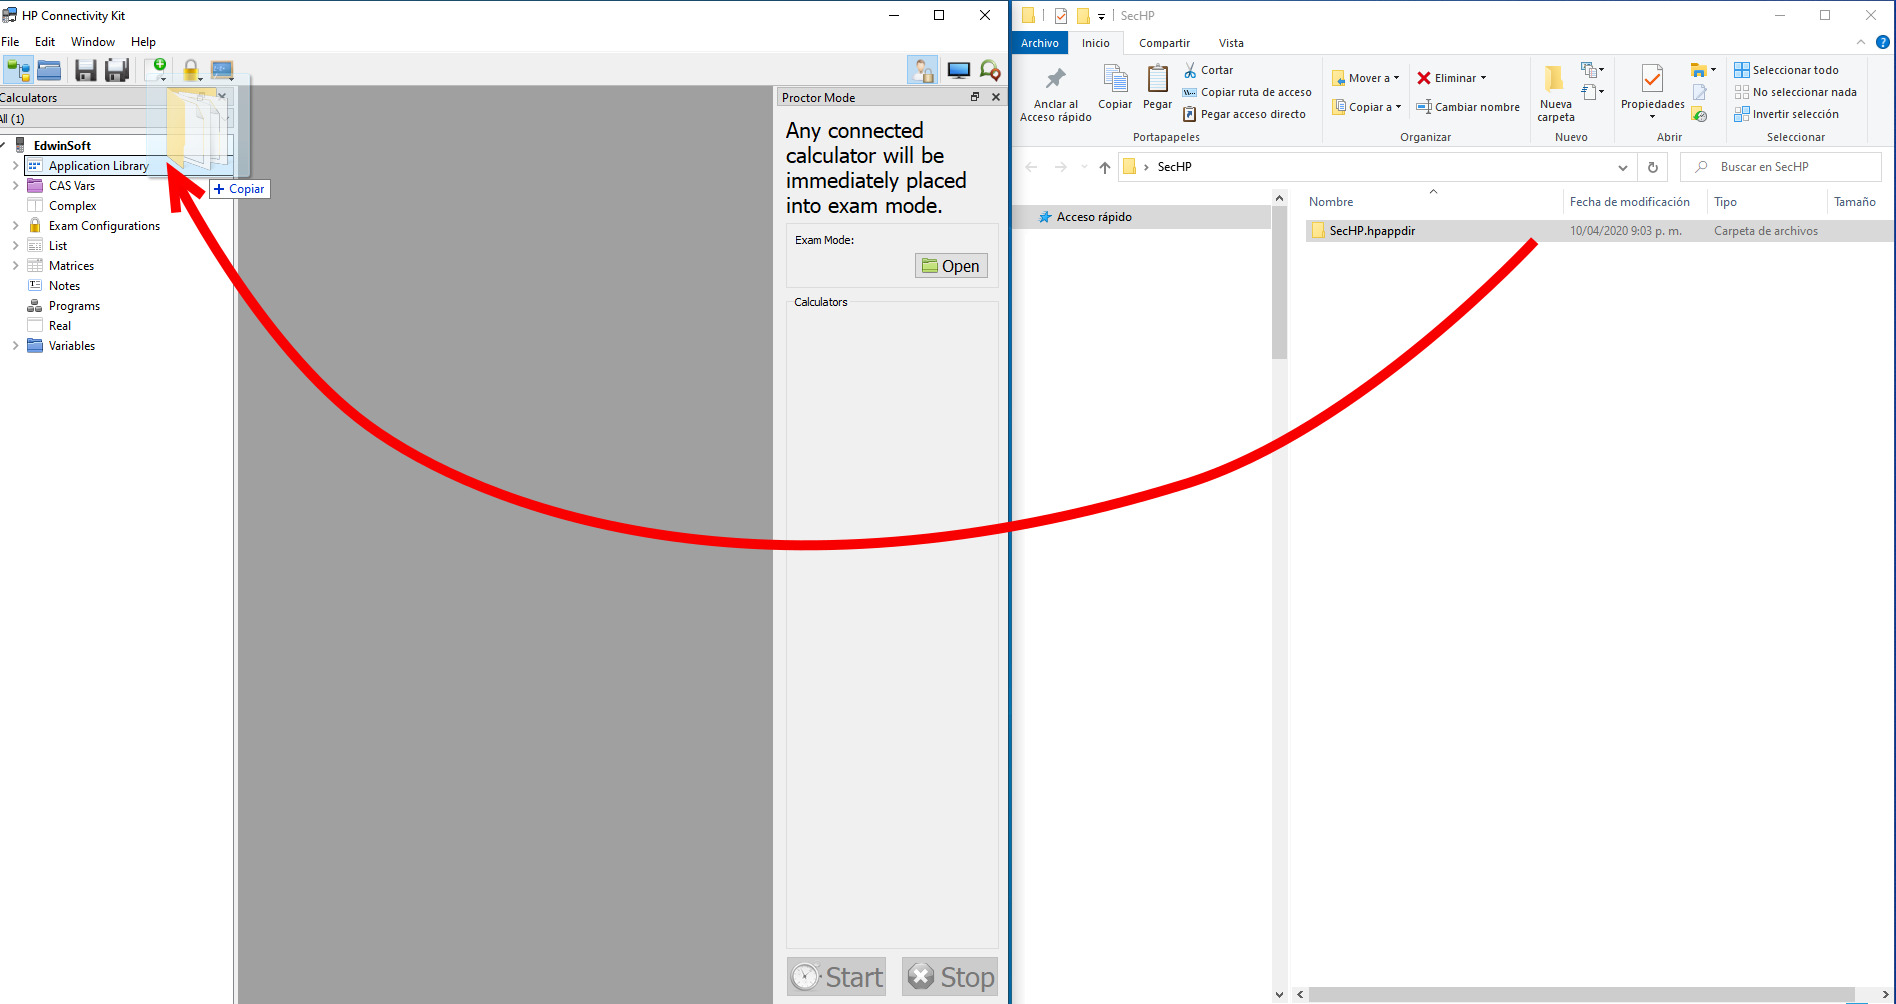
\includegraphics[width=0.7\linewidth]{imagenes/instalacion}	
\end{figure}
\section{Funcionamiento del programa.}
A continuación se describe los comandos y menús que se despliegan al ejecutar el programa como aplicación o desde Home.

\subsection{Aplicación.}
Al ejecutar el programa desde la biblioteca de aplicaciones (Ver Figura \ref{fig:ejeAppBibl}), aparecerá la pantalla de inicio mostrada en la Figura \ref{fig:inicio}. 
\begin{figure}[H]
	\centering
	\caption{Ejecución de SecHP desde la biblioteca de aplicaciones.}
	\label{fig:ejeAppBibl}
	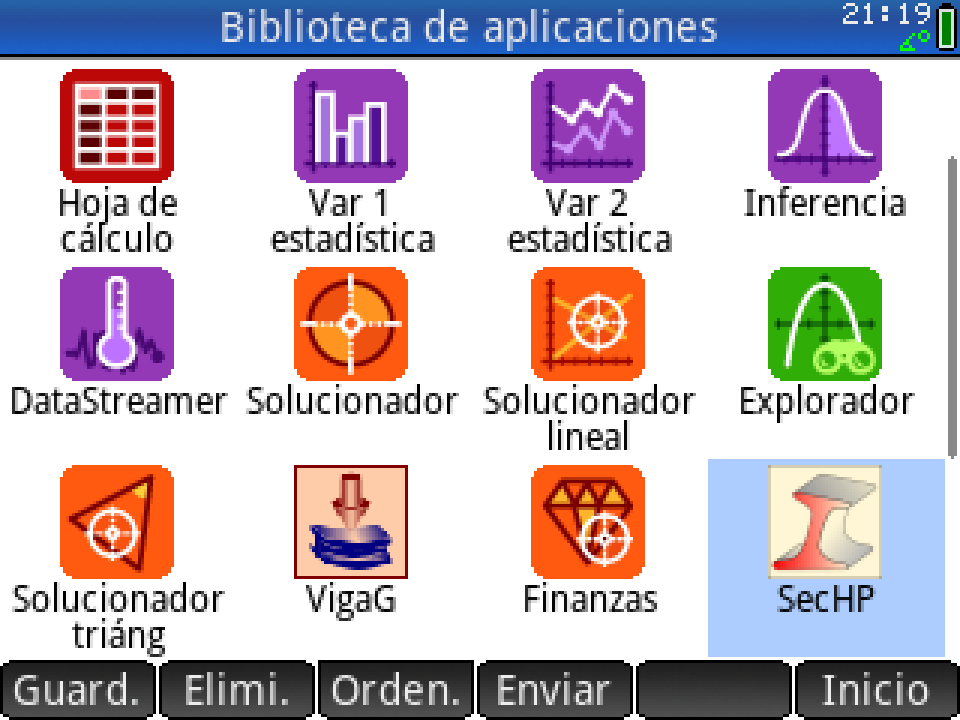
\includegraphics[width=0.45\linewidth]{imagenes/app}	
\end{figure}
\begin{figure}[H]
	\centering
	\caption{Pantalla de inicio de la aplicación SecHP.}
	\label{fig:inicio}
	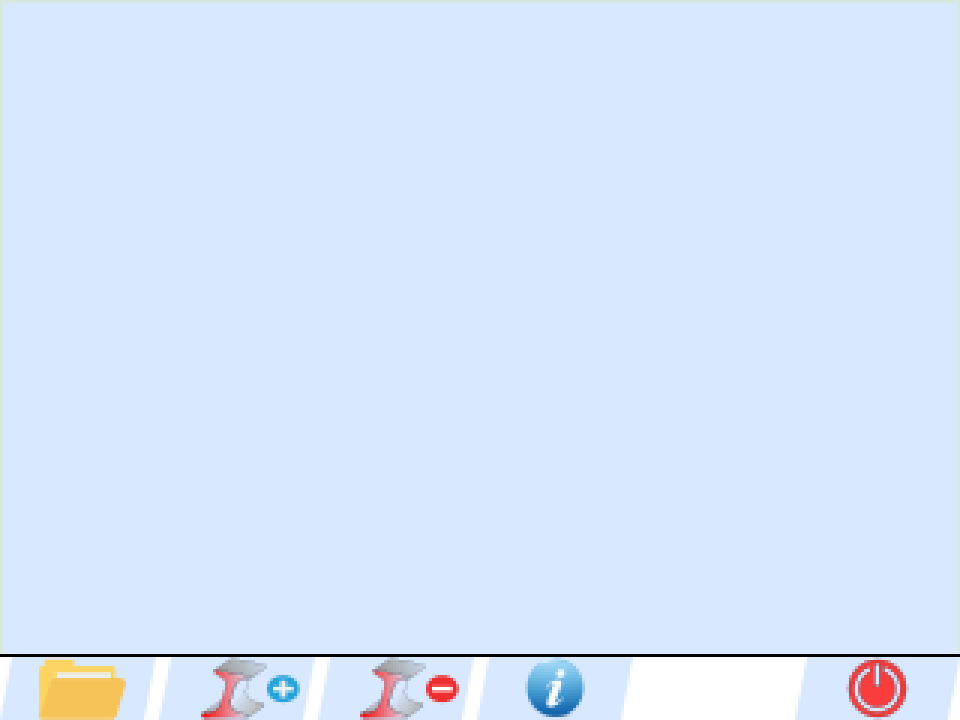
\includegraphics[width=0.45\linewidth]{imagenes/pantallaInicio}	
\end{figure}
%Los menús de le la aplicación se detallan a continuación.
\subsubsection{Menú de la aplicación.}
Al ejecutarse la aplicación el primer menú que aparece es el mostrado en la Tabla \ref{tab:menuInicio}. 
\begin{table}[H]
	\caption{Menú de inicio.}
	\label{tab:menuInicio}
	\begin{tabular}{>{\centering}m{2cm}>{\raggedright}m{14cm}}
		\toprule 
		\textbf{Menú} & \multicolumn{1}{c}{\textbf{Descripción}} \tabularnewline
		\midrule 
		
\includegraphics{imagenes/men_abrir}
		& Abre un archivo previamente guardado, el cual contiene la información de la sección. \tabularnewline
		\cmidrule(lr){1-2}
		
\includegraphics{imagenes/men_nuevo} & Crea nuevos datos para una sección.\tabularnewline
		\cmidrule(lr){1-2}
		
\includegraphics{imagenes/men_eliminar}& Elimina un archivo previamente creado.\tabularnewline
		\cmidrule(lr){1-2}
		
\includegraphics{imagenes/men_about}& Muestra la información del autor y de la versión del programa.\tabularnewline
		\cmidrule(lr){1-2}
		
\includegraphics{imagenes/men_salir}& Sale del programa.\tabularnewline
		\bottomrule
	\end{tabular}
\end{table}
Al dar clic en el menú abrir 
\includegraphics{imagenes/men_abrir}, se despliega la plantilla de entrada de datos mostrada en la Figura \ref{fig:archivoabrir}. Si selecciona ``Canc.''  el programa no creará nuevos datos y volverá al menú principal.
\begin{figure}[H]
	\centering
	\caption[Archivo a Abrir.]{Archivo a Abrir.}
	\label{fig:archivoabrir}
	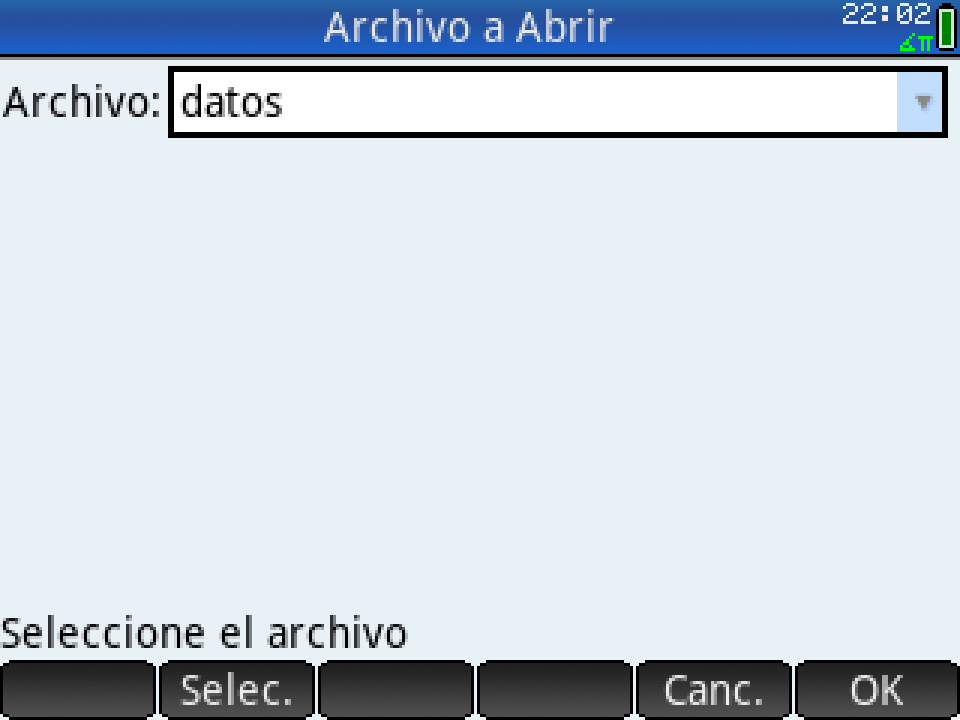
\includegraphics[width=0.45\linewidth]{imagenes/archivoAbrir}
\end{figure}
Al dar clic en el menú nuevos datos 
\includegraphics{imagenes/men_nuevo}, se despliega la plantilla de entrada de datos mostrada en la Figura \ref{fig:datosseccion}. Si selecciona ``Canc.'' el programa tomará los datos mostrados por defecto.

\begin{figure}[H]
	\centering
	\caption[Datos de la Viga.]{Configuración del programa.}
	\label{fig:datosseccion}
	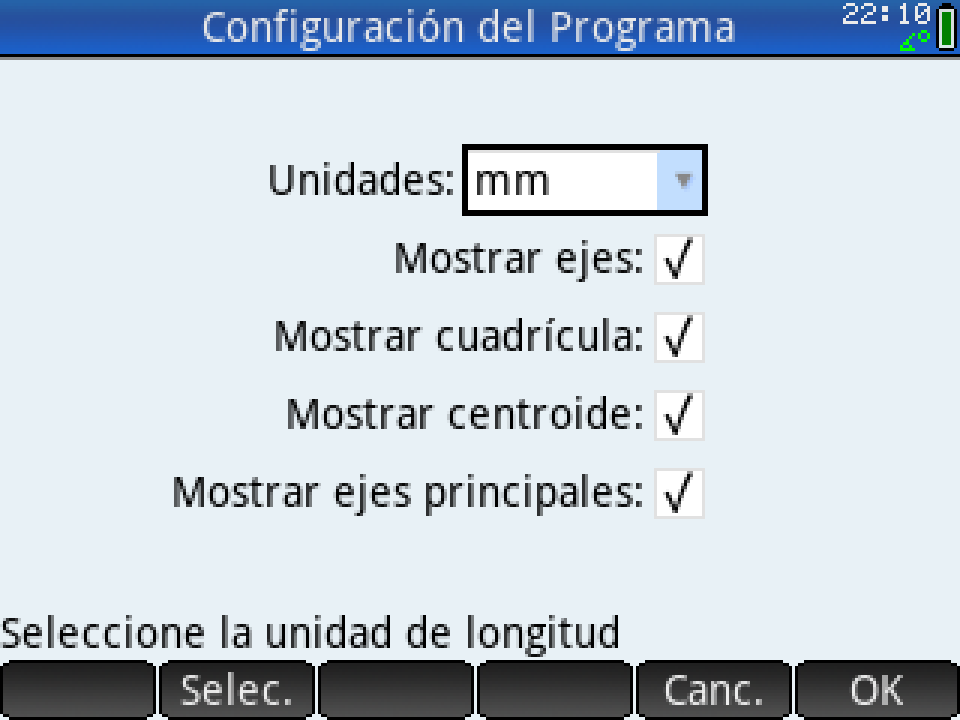
\includegraphics[width=0.45\linewidth]{imagenes/datosSeccion}
\end{figure}
La información de cada una de las entradas es la siguiente:
\begin{description}
	\item[Unidades:] Selección de las unidades de longitud que se trabajará la sección, las posibilidades son: m, cm, mm, ft y in.
	\item[Mostrar ejes:] Si se selecciona mostrará los ejes de referencia x vs. y. 
	\item[Mostrar cuadricula:] Si se selecciona mostrará una cuadrícula de referencia.
	\item[Mostrar centroide:]  Si se selecciona mostrará la ubicación del centroide.
	\item[Mostrar ejes principales:]  Si se selecciona mostrará los ejes principales de los momentos de inercia.
\end{description}
Al dar clic en el menú nuevos datos 
\includegraphics{imagenes/men_eliminar}, se despliega la plantilla de entrada de datos mostrada en la Figura \ref{fig:archivoeliminar}. Si selecciona Canc. el programa no eliminará ningún archivo y volverá al menú principal.
\begin{figure}[H]
	\centering
	\caption[Archivo a Eliminar]{Archivo a Eliminar.}
	\label{fig:archivoeliminar}
	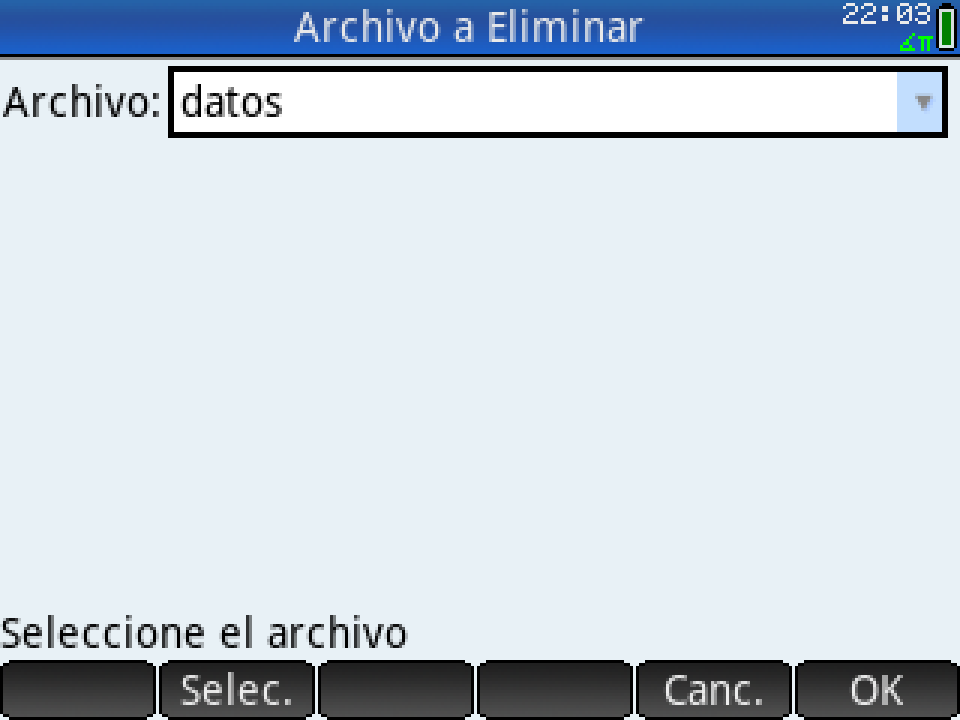
\includegraphics[width=0.45\linewidth]{imagenes/archivoEliminar}
\end{figure}
\subsubsection{Menú secundario.}
Al crear una nueva sección o al abrir un archivo de datos, se mostrara el menú mostrado en la Tabla \ref{tab:menuSecundario}. 
\begin{table}[H]
	\caption{Menú secundario.}
	\label{tab:menuSecundario}
	\begin{tabular}{>{\centering}m{2cm}>{\raggedright}m{14cm}}
		\toprule 
		\textbf{Menú} & \multicolumn{1}{c}{\textbf{Descripción}} \tabularnewline
		\midrule 
		
\includegraphics{imagenes/men_figuras}
		& Despliega el menú de figuras.\tabularnewline	
		\cmidrule(lr){1-2}
		
\includegraphics{imagenes/men_guardar}& Guarda los datos de la sección bajo un nombre dado.\tabularnewline
		\cmidrule(lr){1-2}
		
\includegraphics{imagenes/men_editar}& Despliega el menú de edición.\tabularnewline
		\cmidrule(lr){1-2}
		
\includegraphics{imagenes/men_home}& Se devuelve al menú principal, dando la opción de guardar los datos.\tabularnewline
		\cmidrule(lr){1-2}
		
\includegraphics{imagenes/men_cfg} & Despliega el menú de configuración.\tabularnewline
		\cmidrule(lr){1-2}
		
\includegraphics{imagenes/men_aceptar}& Muestra los cálculos de la sección.\tabularnewline
		\bottomrule
	\end{tabular}
\end{table}
Al dar clic en el menú nuevos datos 
\includegraphics{imagenes/men_guardar}, se despliega la plantilla de entrada de datos mostrada en la Figura \ref{fig:guardar}. Si selecciona ``Canc.'' el programa no guardará los datos.
\begin{figure}[H]
	\centering
	\caption[Plantilla guardar datos.]{Plantilla guardar datos.}
	\label{fig:guardar}
	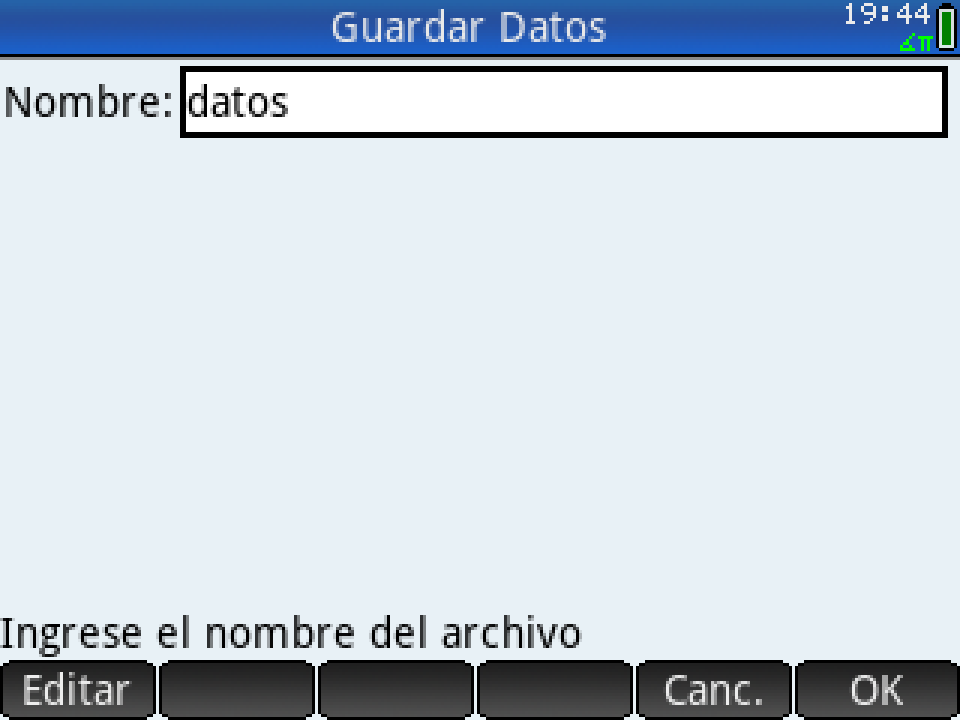
\includegraphics[width=0.45\linewidth]{imagenes/guardar}
\end{figure}
\subsubsection{Menú de figuras.}
En el menú de figuras se agregan nuevas figuras geométricas o perfiles, las opciones  se muestran en la Tabla \ref{tab:menuFiguras}.
\begin{table}[H]
	\caption{Menú de figuras}
	\label{tab:menuFiguras}
	\begin{tabular}{>{\centering}m{2cm}>{\raggedright}m{14cm}}
		\toprule 
		\textbf{Menú} & \multicolumn{1}{c}{\textbf{Descripción}} \tabularnewline
		\midrule 
		
\includegraphics{imagenes/men_circulo}
		& Ingreso de un circulo.\tabularnewline
		\cmidrule(lr){1-2}
		
\includegraphics{imagenes/men_sector} &Ingreso de un sector circular. \tabularnewline
		\cmidrule(lr){1-2}
		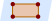
\includegraphics{imagenes/men_rectangulo}&Ingreso de un rectángulo. \tabularnewline
		\cmidrule(lr){1-2}
		
\includegraphics{imagenes/men_poligono}&Ingreso de un polígono. \tabularnewline
		\cmidrule(lr){1-2}
		
\includegraphics{imagenes/men_perfil}& Ingreso de un perfil.\tabularnewline
		\cmidrule(lr){1-2}
		
\includegraphics{imagenes/men_volver}& Retorna al menú secundario \tabularnewline
		\bottomrule
	\end{tabular}
\end{table}
Al dar clic en el menú de círculo 
\includegraphics{imagenes/men_circulo}, se despliega la plantilla de entrada de datos mostrada en la Figura \ref{fig:circulo}, los datos solicitados son el signo del área, las coordenadas del centro y el radio.

\begin{figure}[H]
	\centering
	\caption[Plantilla ingreso datos del círculo.]{Plantilla ingreso datos del círculo.}
	\label{fig:circulo}
	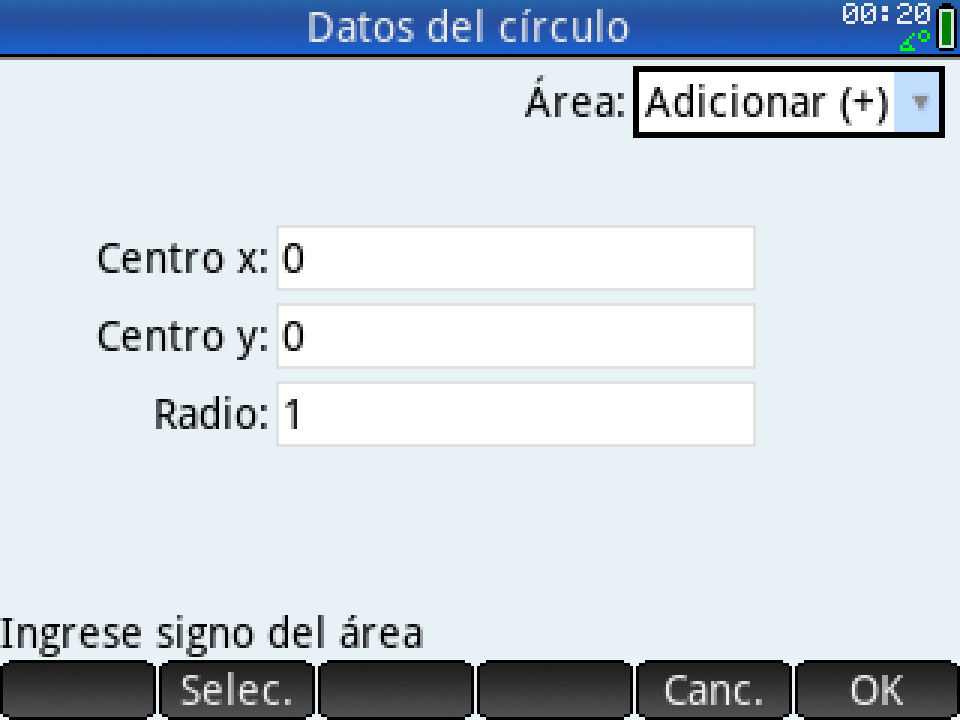
\includegraphics[width=0.45\linewidth]{imagenes/ingresoCirculo}
\end{figure}
Al dar clic en el menú de sector circular 
\includegraphics{imagenes/men_sector}, se despliega la plantilla de entrada de datos mostrada en la Figura \ref{fig:sector}, los datos solicitados son el signo del área, las coordenadas del centro, el radio, ángulo inicial y ángulo final.

\begin{figure}[H]
	\centering
	\caption[Plantilla ingreso datos del sector circular.]{Plantilla ingreso datos del sector circular.}
	\label{fig:sector}
	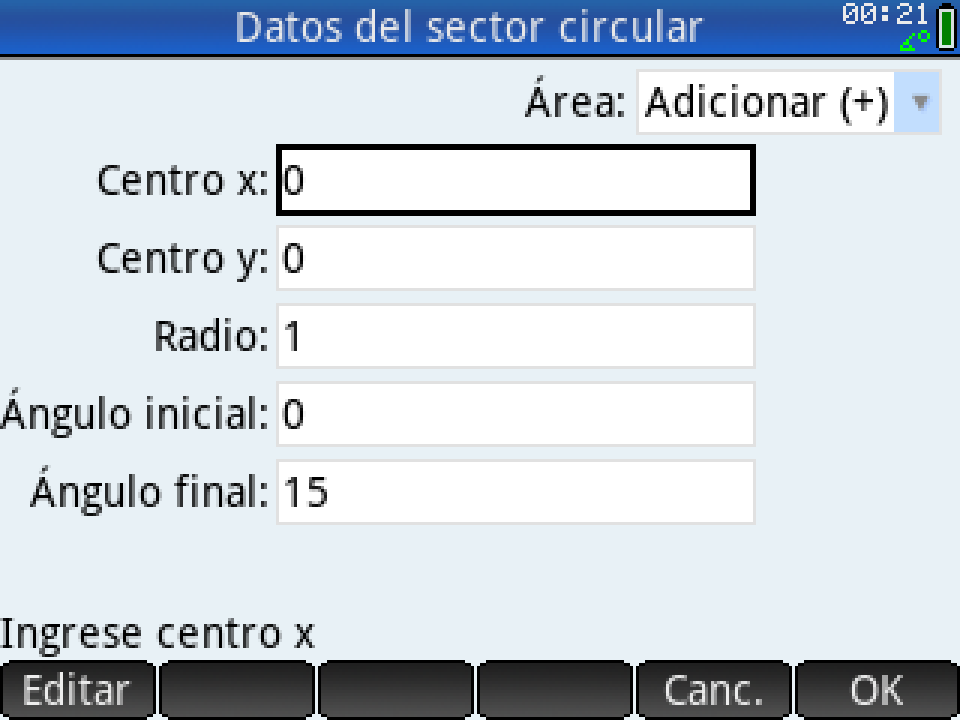
\includegraphics[width=0.45\linewidth]{imagenes/ingresoSectorCircular}
\end{figure}

Al dar clic en el menú de rectángulo 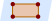
\includegraphics{imagenes/men_rectangulo}, se despliega la plantilla de entrada de datos mostrada en la Figura \ref{fig:rectangulo}, los datos solicitados son el signo del área, las coordenadas del punto izquierdo inferior y las coordenadas del punto derecho superior.

\begin{figure}[H]
	\centering
	\caption[Plantilla ingreso datos del rectángulo.]{Plantilla ingreso datos del rectángulo.}
	\label{fig:rectangulo}
	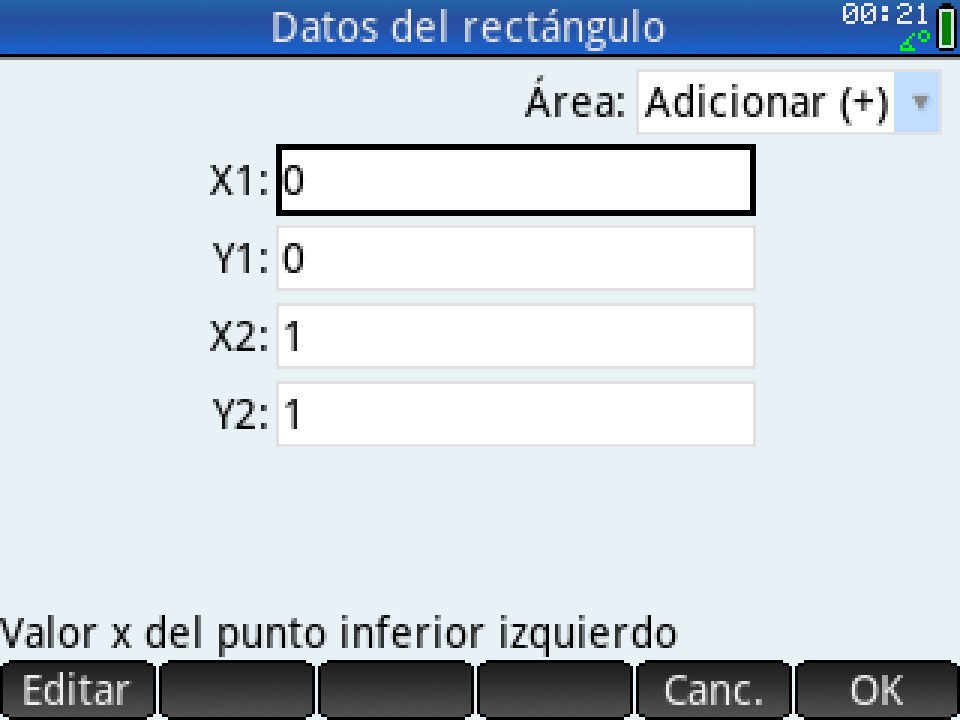
\includegraphics[width=0.45\linewidth]{imagenes/ingresoRectangulo}
\end{figure}

Al dar clic en el menú de polígono 
\includegraphics{imagenes/men_poligono}, se despliegan dos plantillas de entrada de datos mostradas en las Figura \ref{fig:pol1} y \ref{fig:pol2}, en la primera plantilla se ingresa el signo del área, y en la segunda plantilla se ingresa una matriz con los puntos consecutivos de coordenadas del polígono, estos puntos pueden ingresarse en sentido horario o antihorario.

\begin{figure}[H]
	\centering
	\caption[Plantilla ingreso signo del polinomio.]{Plantilla ingreso signo del polinomio.}
	\label{fig:pol1}
	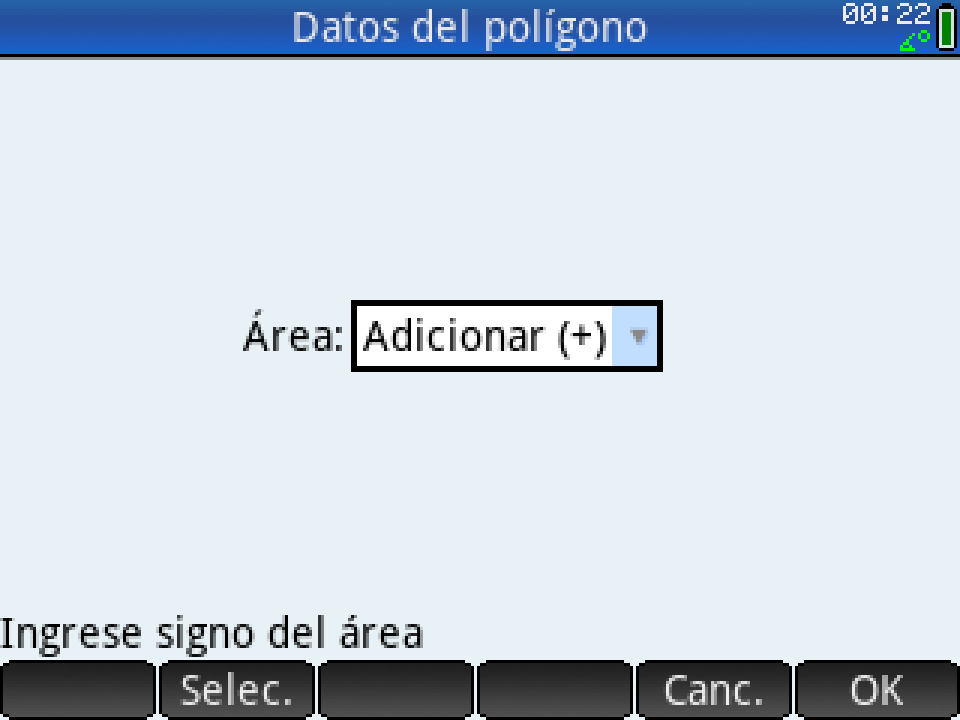
\includegraphics[width=0.45\linewidth]{imagenes/ingresoPolSigno}
\end{figure}
\begin{figure}[H]
	\centering
	\caption[Plantilla ingreso puntos del polinomio.]{Plantilla ingreso puntos del polinomio.}
	\label{fig:pol2}
	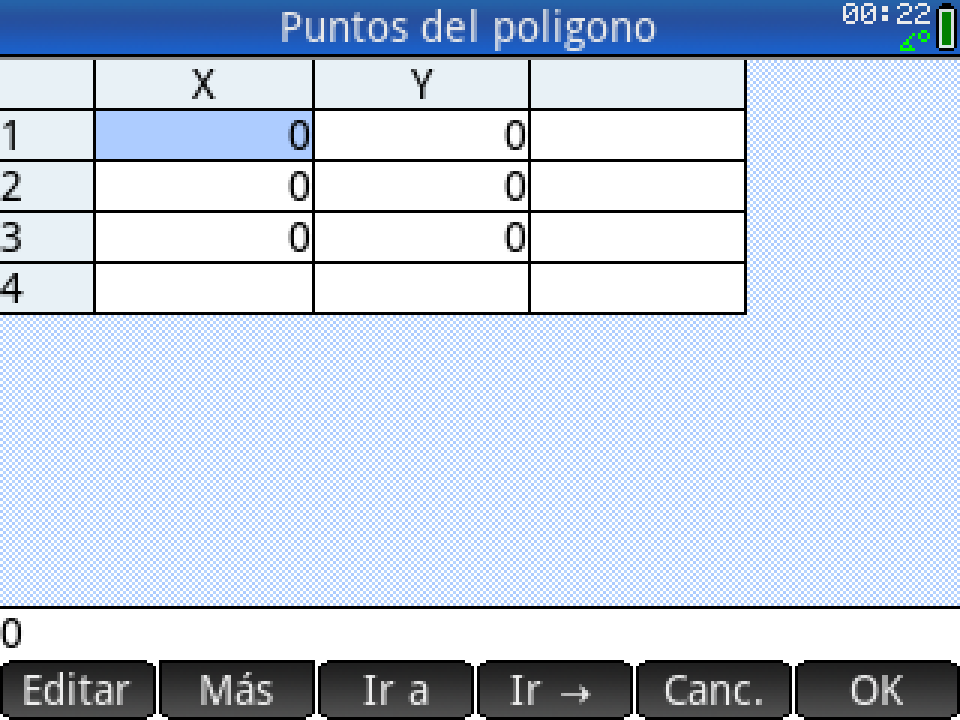
\includegraphics[width=0.45\linewidth]{imagenes/ingresoPolinomio}
\end{figure}

Al dar clic en el menú de perfiles 
\includegraphics{imagenes/men_perfil}, se despliegan dos plantillas de entrada de datos mostradas en las Figura \ref{fig:per1} y \ref{fig:per2}, en la primera plantilla se ingresa el tipo de perfil, que puede ser: Perfil W, Perfil S, Perfil C, Perfil L de lados iguales y Perfil L de lados desiguales, y en la segunda plantilla se seleccionada el perfil de acuerdo al tipo seleccionado, además se ingresa el ángulo de rotación del perfil y el punto donde se ubicará el centroide del perfil.
\begin{figure}[H]
	\centering
	\caption[Plantilla ingreso tipo de perfil.]{Plantilla ingreso tipo de perfil.}
	\label{fig:per1}
	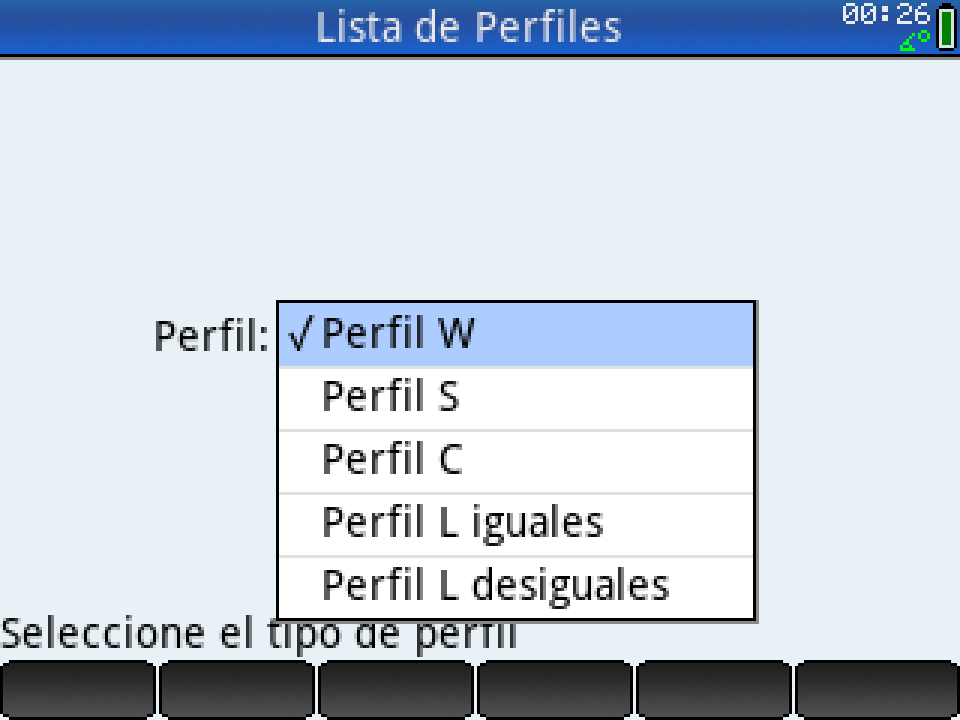
\includegraphics[width=0.45\linewidth]{imagenes/ingresoTipoPerfil}
\end{figure}
\begin{figure}[H]
	\centering
	\caption[Plantilla ingreso de perfil.]{Plantilla ingreso de perfil.}
	\label{fig:per2}
	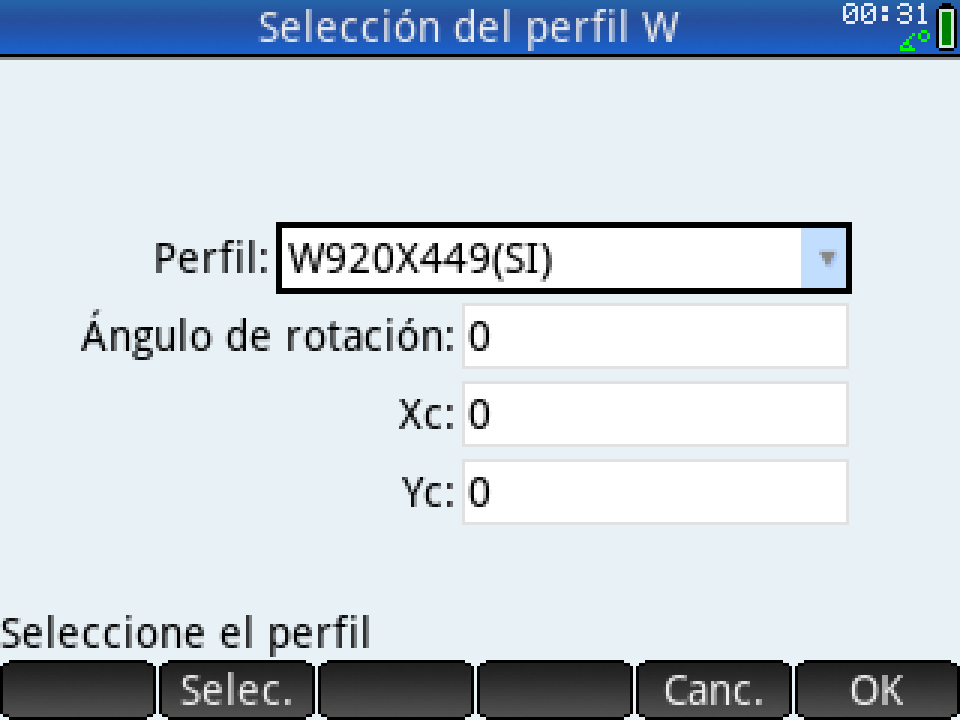
\includegraphics[width=0.45\linewidth]{imagenes/ingresoPerfil}
\end{figure}
\subsubsection{Menú de edición ítem.}
El menú de edición de ítem se muestra cuando se está editando las figuras geométricas o perfiles y se interactúa con cada uno de los menús que se muestran en la Tabla \ref{tab:menuEdicionItem}.

\begin{table}[H]
	\caption{Menú de edición ítem.}
	\label{tab:menuEdicionItem}
	\begin{tabular}{>{\centering}m{2cm}>{\raggedright}m{14cm}}
		\toprule 
		\textbf{Menú} & \multicolumn{1}{c}{\textbf{Descripción}} \tabularnewline
		\midrule 
		
\includegraphics{imagenes/men_anterior}
		& Muestra el ítem anterior.\tabularnewline
		\cmidrule(lr){1-2}
		
\includegraphics{imagenes/men_siguiente} & Muestra el ítem siguiente.\tabularnewline
		\cmidrule(lr){1-2}
		
\includegraphics{imagenes/men_editar}& Edita el ítem seleccionado.\tabularnewline
		\cmidrule(lr){1-2}
		
\includegraphics{imagenes/men_eliminar_dato}& Elimina el ítem seleccionado.\tabularnewline
		\cmidrule(lr){1-2}
		
\includegraphics{imagenes/men_info_figura}& Muestra la información del ítem seleccionado.\tabularnewline
		\cmidrule(lr){1-2}
		
\includegraphics{imagenes/men_volver}& Retorna al menú de secundario.\tabularnewline
		\bottomrule
	\end{tabular}
\end{table}

Al dar clic sobre el menú de configuración 
\includegraphics{imagenes/men_cfg}, se presenta la configuración del programa mostrado en la Figura \ref{fig:datosseccion}.

\subsubsection{Menú de Resultados.}
El menú de resultados se muestra cuando se da clic en el menú 
\includegraphics{imagenes/men_aceptar} y se muestra el menú que se describe en la Tabla \ref{tab:menuResultados}.

\begin{table}[H]
	\caption{Menú de edición ítem.}
	\label{tab:menuResultados}
	\begin{tabular}{>{\centering}m{2cm}>{\raggedright}m{14cm}}
		\toprule 
		\textbf{Menú} & \multicolumn{1}{c}{\textbf{Descripción}} \tabularnewline
		\midrule 
		\includegraphics{imagenes/men_tabla}
		& Muestra los resultados de los cálculos de cada una de las figuras en formato de una tabla.\tabularnewline
		\cmidrule(lr){1-2}
		\includegraphics{imagenes/men_resultados} & Muestra los resultados finales de la sección.\tabularnewline
		\cmidrule(lr){1-2}
		\includegraphics{imagenes/men_volver}& Retorna al menú de secundario.\tabularnewline
		\bottomrule
	\end{tabular}
\end{table}
\subsection{CAL(archivo).}
El comando \verb|CAL(archivo)| calcula la sección con la información obtenida en el argumento \verb|archivo|. El formato del argumento es el siguiente:

$$archivo=\{Unidades, Figuras\}$$
\begin{car}[Unidades:\{n\}]{}
	Donde n (el rango es de 1 a 5) es un número entero que indica la selección de la unidad escogida como se muestra en la Tabla \ref{tab:longitud}.
	\begin{table}[H]
		\caption{Unidades disponibles para la longitud.}
		\label{tab:longitud}
		\centering
		\begin{tabular}{>{\centering}m{1cm}>{\centering}m{2cm}}
			\toprule 
			\multicolumn{1}{c}{\textbf{n}}& \multicolumn{1}{c}{\textbf{Unidad}} \tabularnewline
			\midrule 
			1
			& $m$ \tabularnewline
			\cmidrule(lr){1-2}
			2
			& $cm$ \tabularnewline
			\cmidrule(lr){1-2}
			3
			& $mm$ \tabularnewline
			\cmidrule(lr){1-2}
			4
			& $ft$ \tabularnewline
			\cmidrule(lr){1-2}
			5
			& $in$ \tabularnewline
			\bottomrule
		\end{tabular}
	\end{table}
\end{car}
\begin{car}[Figuras:\{\{Círculos\}, \{Sectores Circulares\}, \{Rectángulos\}, \{Polígonos\}, \{Perfiles\}\}]{}
	\begin{description}
		\item[Círculos:] \{\{Datos\},\{Cálculos\},Signo\}.
		\begin{description}
			\item[Datos:] \{($Centro_{x}$,$Centro_{y}$), radio\}.
			\item[Cálculos:]\{Área,Centroide,Ixxc,Iyyc,Ixyc,Ixx,Iyy,Ixy,MinMax\}, inicialmente esta lista está vacía, pero el programa acá guarda los cálculos realizados de la figura.
			\begin{description}
				\item[Área:] Área de la figura.
				\item[Centroide:] Centroide de la figura $(x_{c},y_{c})$.
				\item[Ixxc:] Momento de inercia con respecto al eje x centroidal.
				\item[Iyyc:] Momento de inercia con respecto al eje y centroidal.
				\item[Ixyc:] Producto de inercia con respecto al eje x y al eje y centroidal.
				\item[Ixx:] Momento de inercia con respecto al eje x de referencia.
				\item[Iyy:] Momento de inercia con respecto al eje y de referencia.
				\item[Ixy:] Producto de inercia con respecto al eje x y al eje y de referencia.
				\item[MinMax:] Lista con el punto máximo y mínimo de la figura, esta información es usada para realizar la gráfica \{$(min_{x},min_{y})$,$(max_{x},max_{y})$\}.
			\end{description}
			\item[Signo: n.] Donde n(el rango es de 1 a 2) corresponde al signo del área, si es una adición a una sustracción. 1 el área es positiva y 2 el área es negativa.
		\end{description}
		\item[Sectores Circulares:] \{\{Datos\},\{Cálculos\},Signo\}.
		\begin{description}
			\item[Datos:] \{($Centro_{x}$,$Centro_{y}$), radio, ángulo inicial, ángulo final\}.
			\item[Cálculos:]\{Área,Centroide,Ixxc,Iyyc,Ixyc,Ixx,Iyy,Ixy,MinMax\}, inicialmente esta lista está vacía, pero el programa acá guarda los cálculos realizados de la figura.
			\begin{description}
				\item[Área:] Área de la figura.
				\item[Centroide:] Centroide de la figura $(x_{c},y_{c})$.
				\item[Ixxc:] Momento de inercia con respecto al eje x centroidal.
				\item[Iyyc:] Momento de inercia con respecto al eje y centroidal.
				\item[Ixyc:] Producto de inercia con respecto al eje x y al eje y centroidal.
				\item[Ixx:] Momento de inercia con respecto al eje x de referencia.
				\item[Iyy:] Momento de inercia con respecto al eje y de referencia.
				\item[Ixy:] Producto de inercia con respecto al eje x y al eje y de referencia.
				\item[MinMax:] Lista con el punto máximo y mínimo de la figura, esta información es usada para realizar la gráfica \{$(min_{x},min_{y})$,$(max_{x},max_{y})$\}.
			\end{description}
			\item[Signo: n.] Donde n(el rango es de 1 a 2) corresponde al signo del área, si es una adición a una sustracción. 1 el área es positiva y 2 el área es negativa.
		\end{description}
		\item[Rectángulos:] \{\{Datos\},\{Cálculos\},Signo\}.
		\begin{description}
			\item[Datos:] \{($P1_{x}$,$P1_{y}$),($P2_{x}$,$P2_{y}$)\}, coordenadas del punto inferior izquierdo (P1) y el punto superior derecho (P2).
			\item[Cálculos:]\{Área,Centroide,Ixxc,Iyyc,Ixyc,Ixx,Iyy,Ixy,MinMax\}, inicialmente esta lista está vacía, pero el programa acá guarda los cálculos realizados de la figura.
			\begin{description}
				\item[Área:] Área de la figura.
				\item[Centroide:] Centroide de la figura $(x_{c},y_{c})$.
				\item[Ixxc:] Momento de inercia con respecto al eje x centroidal.
				\item[Iyyc:] Momento de inercia con respecto al eje y centroidal.
				\item[Ixyc:] Producto de inercia con respecto al eje x y al eje y centroidal.
				\item[Ixx:] Momento de inercia con respecto al eje x de referencia.
				\item[Iyy:] Momento de inercia con respecto al eje y de referencia.
				\item[Ixy:] Producto de inercia con respecto al eje x y al eje y de referencia.
				\item[MinMax:] Lista con el punto máximo y mínimo de la figura, esta información es usada para realizar la gráfica \{$(min_{x},min_{y})$,$(max_{x},max_{y})$\}.
			\end{description}
			\item[Signo: n.] Donde n(el rango es de 1 a 2) corresponde al signo del área, si es una adición a una sustracción. 1 el área es positiva y 2 el área es negativa.
		\end{description}
		\item[Polígonos:] \{\{Datos\},\{Cálculos\},Signo\}.
		\begin{description}
			\item[Datos:]$\{\left[\left[x_{1},y_{1}\right],\left[x_{2},y_{2}\right],\dots,\left[x_{n},y_{n}\right]\right]\}$
			, Matriz con las coordenadas de los puntos consecutivos que definen al polígono.
			\item[Cálculos:]\{Área,Centroide,Ixxc,Iyyc,Ixyc,Ixx,Iyy,Ixy,MinMax\}, inicialmente esta lista está vacía, pero el programa acá guarda los cálculos realizados de la figura.
			\begin{description}
				\item[Área:] Área de la figura.
				\item[Centroide:] Centroide de la figura $(x_{c},y_{c})$.
				\item[Ixxc:] Momento de inercia con respecto al eje x centroidal.
				\item[Iyyc:] Momento de inercia con respecto al eje y centroidal.
				\item[Ixyc:] Producto de inercia con respecto al eje x y al eje y centroidal.
				\item[Ixx:] Momento de inercia con respecto al eje x de referencia.
				\item[Iyy:] Momento de inercia con respecto al eje y de referencia.
				\item[Ixy:] Producto de inercia con respecto al eje x y al eje y de referencia.
				\item[MinMax:] Lista con el punto máximo y mínimo de la figura, esta información es usada para realizar la gráfica \{$(min_{x},min_{y})$,$(max_{x},max_{y})$\}.
			\end{description}
			\item[Signo: n.] Donde n(el rango es de 1 a 2) corresponde al signo del área, si es una adición a una sustracción. 1 el área es positiva y 2 el área es negativa.
		\end{description}
		\item[Perfiles:] \{\{Datos\},\{Cálculos\},\{Puntos\}\}.
		\begin{description}
			\item[Datos:]\{\{i,j\},$\theta$,$x_{c}$,$y_{c}$\}, i corresponde a un entero que identifica el tipo de perfil (1=Perfil W, 2=Perfil S, 3=Perfil C, 4=Perfil L de lados iguales, 5=Perfil L de lados desiguales), j corresponde a la ubicación del perfil en la lista, ver Tabla \ref{tab:perfilesDisponibles}, $\theta$ corresponde al ángulo de rotación del perfil, $x_{c}$ es la ubicación del centroide en x, y $y_{c}$ es la ubicación del centroide en y.
			\item[Cálculos:]\{Área,Centroide,Ixxc,Iyyc,Ixyc,Ixx,Iyy,Ixy,MinMax\}, inicialmente esta lista está vacía, pero el programa acá guarda los cálculos realizados de la figura.
			\begin{description}
				\item[Área:] Área de la figura.
				\item[Centroide:] Centroide de la figura $(x_{c},y_{c})$.
				\item[Ixxc:] Momento de inercia con respecto al eje x centroidal.
				\item[Iyyc:] Momento de inercia con respecto al eje y centroidal.
				\item[Ixyc:] Producto de inercia con respecto al eje x y al eje y centroidal.
				\item[Ixx:] Momento de inercia con respecto al eje x de referencia.
				\item[Iyy:] Momento de inercia con respecto al eje y de referencia.
				\item[Ixy:] Producto de inercia con respecto al eje x y al eje y de referencia.
				\item[MinMax:] Lista con el punto máximo y mínimo de la figura, esta información es usada para realizar la gráfica \{$(min_{x},min_{y})$,$(max_{x},max_{y})$\}.
			\end{description}
			\item[Puntos:] $\{\left[\left[x_{1},y_{1}\right],\left[x_{2},y_{2}\right],\dots,\left[x_{n},y_{n}\right]\right]\}$, Matriz con las coordenadas de los puntos consecutivos que definen el controno del perfil, esta lista inicialmente es vacía y el programa la crea de acuerdo a las dimensiones del perfil.
		\end{description}
	\end{description}
\end{car}
\subsubsection{Ejemplo de sección.}
La Figura \ref{fig:seccionEjemplo} define una sección compuesta por tres figuras, un polígono y un sector circular como áreas positivas, y un circulo con área negativa. Los datos que definen esta sección es la siguiente lista:

\{

\hspace{0.5cm}\{3\},

\hspace{0.5cm}\{

\hspace{1cm}\{

\hspace{1.5cm}\{\{(100,100),50\},\{\},2\}

\hspace{1cm}\},

\hspace{1cm}\{

\hspace{1.5cm}\{\{(100,100),100,90,270\},\{\},1\}

\hspace{1cm}\},

\hspace{1cm}\{\},

\hspace{1cm}\{

\hspace{1.5cm}\{\{[[100,0],[200,0],[350,200],[100,200]]\},\{\},1\}

\hspace{1cm}\},

\hspace{1cm}\{\}

\hspace{0.5cm}\}

\}

\begin{figure}[H]
	\centering
	\caption{Sección de ejemplo}
	\label{fig:seccionEjemplo}
	\begin{tikzpicture}[scale=1]
	
	\draw[->,>=stealth,draw=black] (0pt,0pt) -- (0pt,250pt);
	\node[anchor=east] (c1) at (0pt,250pt){$y$};
	\draw[->,>=stealth,draw=black] (0pt,0pt) -- (400pt,0pt);
	\node[anchor=north] (c2) at (400pt,0pt){$x$};
	\draw[fill=blue] (100pt,0pt) -- ++(100pt,0pt) -- ++(150pt,200pt)-- ++(-250pt,0pt)--cycle;
	\draw[fill=blue] (100pt,200pt) arc (90:270:100pt);
	\draw[fill=white] (100pt,100pt) circle (50pt);
	\node[draw=white,fill=white,scale=0.9] (r1) at (125pt,100pt){$50\,mm$};
	\node[draw=white,fill=white,scale=0.9] (c1) at (50pt,-10pt){$100\,mm$};
	\node[draw=white,fill=white] (c2) at (150pt,-10pt){$100\,mm$};
	\node[draw=white,fill=white] (c3) at (275pt,-10pt){$150\,mm$};
	\draw[draw=gray] (0pt,-15pt)--++(0pt,10pt);
	\draw[draw=gray] (100pt,-15pt)--++(0pt,10pt);
	\draw[draw=gray] (200pt,-15pt)--++(0pt,10pt);
	\draw[draw=gray] (350pt,-15pt)--++(0pt,10pt);

	
	\draw[draw=gray,fill=white] (100pt,100pt)--(r1);
	\draw[draw=gray,fill=white,->,>=stealth'] (r1)--(150pt,100pt);
	
	\draw[draw=gray,fill=white,<-,>=stealth'] (0pt,-10pt)--(c1);
	\draw[draw=gray,fill=white,->,>=stealth'] (c1)--(100pt,-10pt);
	\draw[draw=gray,fill=white,<-,>=stealth'] (100pt,-10pt)--(c2);
	\draw[draw=gray,fill=white,->,>=stealth'] (c2)--(200pt,-10pt);
	\draw[draw=gray,fill=white,<-,>=stealth'] (200pt,-10pt)--(c3);
	\draw[draw=gray,fill=white,->,>=stealth'] (c3)--(350pt,-10pt);
	\end{tikzpicture}
\end{figure}
\subsection{FIG(archivo).}
El comando \verb|FIG(archivo)| genera la figura de la sección que representa los datos que se encuentra en el argumento \verb|archivo|. Para el ejemplo mostrado en la Figura \ref{fig:seccionEjemplo}, la figura generada se muestra en la Figuras \ref{fig:res1} y \ref{fig:res2}.

\begin{figure}[H]
	\centering
	\caption[Generación de la Figura a partir de datos vista 1.]{Generación de la Figura a partir de datos vista 1.}
	\label{fig:res1}
	\includegraphics[width=0.45\linewidth]{imagenes/resultadoFig1}
\end{figure}
\begin{figure}[H]
	\centering
	\caption[Generación de la Figura a partir de datos vista 2.]{Generación de la Figura a partir de datos vista 2.}
	\label{fig:res2}
	\includegraphics[width=0.45\linewidth]{imagenes/resultadoFig2}
\end{figure}
\subsection{TAB(archivo).}
El comando \verb|TAB(archivo)| genera la tabla de cálculos de la sección que representa los datos que se encuentra en el argumento \verb|archivo|. Para el ejemplo mostrado en la Figura \ref{fig:seccionEjemplo}, la tabla generada se muestra en la Figura \ref{fig:tab}.

\begin{figure}[H]
	\centering
	\caption[Generación de la tabla de cálculos.]{Generación de la tabla de cálculos.}
	\label{fig:tab}
	\includegraphics[width=0.45\linewidth]{imagenes/resultadoTAB}
\end{figure}

\subsection{VER().}
El comando \verb|VER()| retorna el número de la versión del programa.

\subsection{PER(n).}
El comando \verb|PER(n)| retorna las propiedades calculadas de un perfil que se seleccionará y las unidades utilizadas dependerá del valor n, donde n (el rango es de 1 a 5) es un número entero que indica la selección de la unidad escogida como se muestra en la Tabla \ref{tab:longitud}.

\section{Comandos de teclado}
Cuando el programa está ejecutándose y se está realizando alguna figura es posible cambiar el aspecto de la figura de acuerdo a la Tabla \ref{tab:teclado}.
\begin{table}[H]
	\caption{Comandos de teclado}
	\label{tab:teclado}
	\begin{tabular}{>{\centering}m{2cm}>{\raggedright}m{14cm}}
		\toprule 
		\textbf{Tecla} & \multicolumn{1}{c}{\textbf{Descripción}} \tabularnewline
		\midrule 
		\hpup
		& Mueve la figura hacia arriba.\tabularnewline
		\cmidrule(lr){1-2}
		\hpdown &Mueve la figura hacia abajo. \tabularnewline
		\cmidrule(lr){1-2}
		\hpleft&Mueve la figura hacia la izquierda. \tabularnewline
		\cmidrule(lr){1-2}
		\hpright&Mueve la figura hacia la derecha. \tabularnewline
		\cmidrule(lr){1-2}
		\hpminus& disminuye el zoom de la figura y la aleja.\tabularnewline
		\cmidrule(lr){1-2}
		\hpplus&  aumenta el zoom de la figura y la acerca. \tabularnewline
		\cmidrule(lr){1-2}
		\hpesc& Realiza un auto-escalado de la figura. \tabularnewline
		\bottomrule
	\end{tabular}
\end{table}  
 También es posible realizar el zoom y el desplazamiento de la figura interactuando con la pantalla táctil. 
\newpage
\appendix
\pagebreak
\hspace{0pt}
\vfill
\begin{center}
	\Huge ANEXOS
\end{center}
\vfill
\hspace{0pt}
\pagebreak
%\appendixpage
\addcontentsline{toc}{section}{ANEXOS}	%
\renewcommand*{\thesection}{\arabic{section}}
\section{Lista de perfiles disponibles en el programa}
{\footnotesize{}}%
\begin{longtable}{clllll}
	\caption{Lista de perfiles disponibles en el programa.\label{tab:perfilesDisponibles}}\\
	\toprule
	\textbf{\footnotesize{}Item} & \textbf{\footnotesize{}Perfil W} & \textbf{\footnotesize{}Perfil S} & \textbf{\footnotesize{}Perfil C} & \textbf{\footnotesize{}Perfil L, lados iguales} & \textbf{\footnotesize{}Perfil L, lados desiguales}\tabularnewline
	\midrule
	\endfirsthead
	\caption[]{Lista de perfiles disponibles en el programa (continuación).}\\ 
	\toprule
	\textbf{\footnotesize{}Item} & \textbf{\footnotesize{}Perfil W} & \textbf{\footnotesize{}Perfil S} & \textbf{\footnotesize{}Perfil C} & \textbf{\footnotesize{}Perfil L, lados iguales} & \textbf{\footnotesize{}Perfil L, lados desiguales}\tabularnewline
	\midrule
	\endhead
	{\footnotesize{}1} & {\footnotesize{}W920\times449(SI)} & {\footnotesize{}S610\times180(SI)} & {\footnotesize{}C380\times74(SI)} & {\footnotesize{}L203\times203\times25.4(SI)} & {\footnotesize{}L203\times152\times25.4(SI)}\tabularnewline
	\midrule 
	{\footnotesize{}2} & {\footnotesize{}W920\times201(SI)} & {\footnotesize{}S610\times158(SI)} & {\footnotesize{}C380\times60(SI)} & {\footnotesize{}L203\times203\times19(SI)} & {\footnotesize{}L203\times152\times19(SI)}\tabularnewline
	\midrule 
	{\footnotesize{}3} & {\footnotesize{}W840\times299(SI)} & {\footnotesize{}S610\times149(SI)} & {\footnotesize{}C380\times50.4(SI)} & {\footnotesize{}L203\times203\times12.7(SI)} & {\footnotesize{}L203\times152\times12.7(SI)}\tabularnewline
	\midrule 
	{\footnotesize{}4} & {\footnotesize{}W840\times176(SI)} & {\footnotesize{}S610\times134(SI)} & {\footnotesize{}C310\times45(SI)} & {\footnotesize{}L152\times152\times25.4(SI)} & {\footnotesize{}L152\times102\times19(SI)}\tabularnewline
	\midrule 
	{\footnotesize{}5} & {\footnotesize{}W760\times257(SI)} & {\footnotesize{}S610\times119(SI)} & {\footnotesize{}C310\times37(SI)} & {\footnotesize{}L152\times152\times19(SI)} & {\footnotesize{}L152\times102\times12.7(SI)}\tabularnewline
	\midrule 
	{\footnotesize{}6} & {\footnotesize{}W760\times147(SI)} & {\footnotesize{}S510\times143(SI)} & {\footnotesize{}C310\times30.8(SI)} & {\footnotesize{}L152\times152\times15.9(SI)} & {\footnotesize{}L152\times102\times9.5(SI)}\tabularnewline
	\midrule 
	{\footnotesize{}7} & {\footnotesize{}W690\times217(SI)} & {\footnotesize{}S510\times128(SI)} & {\footnotesize{}C250\times45(SI)} & {\footnotesize{}L152\times152\times12.7(SI)} & {\footnotesize{}L127\times76\times12.7(SI)}\tabularnewline
	\midrule 
	{\footnotesize{}8} & {\footnotesize{}W690\times125(SI)} & {\footnotesize{}S510\times112(SI)} & {\footnotesize{}C250\times37(SI)} & {\footnotesize{}L152\times152\times9.5(SI)} & {\footnotesize{}L127\times76\times9.5(SI)}\tabularnewline
	\midrule 
	{\footnotesize{}9} & {\footnotesize{}W610\times155(SI)} & {\footnotesize{}S510\times98.2(SI)} & {\footnotesize{}C250\times30(SI)} & {\footnotesize{}L127\times127\times19(SI)} & {\footnotesize{}L127\times76\times6.4(SI)}\tabularnewline
	\midrule 
	{\footnotesize{}10} & {\footnotesize{}W610\times101(SI)} & {\footnotesize{}S460\times104(SI)} & {\footnotesize{}C250\times22.8(SI)} & {\footnotesize{}L127\times127\times15.9(SI)} & {\footnotesize{}L102\times76\times12.7(SI)}\tabularnewline
	\midrule 
	{\footnotesize{}11} & {\footnotesize{}W530\times150(SI)} & {\footnotesize{}S460\times81.4(SI)} & {\footnotesize{}C230\times30(SI)} & {\footnotesize{}L127\times127\times12.7(SI)} & {\footnotesize{}L102\times76\times9.5(SI)}\tabularnewline
	\midrule 
	{\footnotesize{}12} & {\footnotesize{}W530\times92(SI)} & {\footnotesize{}S380\times74(SI)} & {\footnotesize{}C230\times22(SI)} & {\footnotesize{}L127\times127\times9.5(SI)} & {\footnotesize{}L102\times76\times6.4(SI)}\tabularnewline
	\midrule 
	{\footnotesize{}13} & {\footnotesize{}W530\times66(SI)} & {\footnotesize{}S380\times64(SI)} & {\footnotesize{}C230\times19.9(SI)} & {\footnotesize{}L102\times102\times19(SI)} & {\footnotesize{}L89\times64\times12.7(SI)}\tabularnewline
	\midrule 
	{\footnotesize{}14} & {\footnotesize{}W460\times158(SI)} & {\footnotesize{}S310\times74(SI)} & {\footnotesize{}C200\times27.9(SI)} & {\footnotesize{}L102\times102\times15.9(SI)} & {\footnotesize{}L89\times64\times9.5(SI)}\tabularnewline
	\midrule 
	{\footnotesize{}15} & {\footnotesize{}W460\times113(SI)} & {\footnotesize{}S310\times60.7(SI)} & {\footnotesize{}C200\times20.5(SI)} & {\footnotesize{}L102\times102\times12.7(SI)} & {\footnotesize{}L89\times64\times6.4(SI)}\tabularnewline
	\midrule 
	{\footnotesize{}16} & {\footnotesize{}W460\times74(SI)} & {\footnotesize{}S310\times52(SI)} & {\footnotesize{}C200\times17.1(SI)} & {\footnotesize{}L102\times102\times9.5(SI)} & {\footnotesize{}L76\times51\times12.7(SI)}\tabularnewline
	\midrule 
	{\footnotesize{}17} & {\footnotesize{}W460\times52(SI)} & {\footnotesize{}S310\times47.3(SI)} & {\footnotesize{}C180\times18.2(SI)} & {\footnotesize{}L102\times102\times6.4(SI)} & {\footnotesize{}L76\times51\times9.5(SI)}\tabularnewline
	\midrule 
	{\footnotesize{}18} & {\footnotesize{}W410\times114(SI)} & {\footnotesize{}S250\times52(SI)} & {\footnotesize{}C180\times14.6(SI)} & {\footnotesize{}L89\times89\times12.7(SI)} & {\footnotesize{}L76\times51\times6.4(SI)}\tabularnewline
	\midrule 
	{\footnotesize{}19} & {\footnotesize{}W410\times85(SI)} & {\footnotesize{}S250\times37.8(SI)} & {\footnotesize{}C150\times19.3(SI)} & {\footnotesize{}L89\times89\times9.5(SI)} & {\footnotesize{}L64\times51\times9.5(SI)}\tabularnewline
	\midrule 
	{\footnotesize{}20} & {\footnotesize{}W410\times60(SI)} & {\footnotesize{}S200\times34(SI)} & {\footnotesize{}C150\times15.6(SI)} & {\footnotesize{}L89\times89\times6.4(SI)} & {\footnotesize{}L64\times51\times6.4(SI)}\tabularnewline
	\midrule 
	{\footnotesize{}21} & {\footnotesize{}W410\times46.1(SI)} & {\footnotesize{}S200\times27.4(SI)} & {\footnotesize{}C150\times12.2(SI)} & {\footnotesize{}L76\times76\times12.7(SI)} & {\footnotesize{}L8\times6\times1(US)}\tabularnewline
	\midrule 
	{\footnotesize{}22} & {\footnotesize{}W410\times38.8(SI)} & {\footnotesize{}S150\times25.7(SI)} & {\footnotesize{}C130\times13(SI)} & {\footnotesize{}L76\times76\times9.5(SI)} & {\footnotesize{}L8\times6\times3\textfractionsolidus 4(US)}\tabularnewline
	\midrule 
	{\footnotesize{}23} & {\footnotesize{}W360\times551(SI)} & {\footnotesize{}S150\times18.6(SI)} & {\footnotesize{}C130\times10.4(SI)} & {\footnotesize{}L76\times76\times6.4(SI)} & {\footnotesize{}L8\times6\times1\textfractionsolidus 2(US)}\tabularnewline
	\midrule 
	{\footnotesize{}24} & {\footnotesize{}W360\times216(SI)} & {\footnotesize{}S130\times15(SI)} & {\footnotesize{}C100\times10.8(SI)} & {\footnotesize{}L64\times64\times12.7(SI)} & {\footnotesize{}L6\times4\times3\textfractionsolidus 4(US)}\tabularnewline
	\midrule 
	{\footnotesize{}25} & {\footnotesize{}W360\times122(SI)} & {\footnotesize{}S100\times14.1(SI)} & {\footnotesize{}C100\times8(SI)} & {\footnotesize{}L64\times64\times9.5(SI)} & {\footnotesize{}L6\times4\times1\textfractionsolidus 2(US)}\tabularnewline
	\midrule 
	{\footnotesize{}26} & {\footnotesize{}W360\times101(SI)} & {\footnotesize{}S100\times11.5(SI)} & {\footnotesize{}C75\times8.9(SI)} & {\footnotesize{}L64\times64\times6.4(SI)} & {\footnotesize{}L6\times4\times3\textfractionsolidus 8(US)}\tabularnewline
	\midrule 
	{\footnotesize{}27} & {\footnotesize{}W360\times79(SI)} & {\footnotesize{}S75\times11.2(SI)} & {\footnotesize{}C75\times7.4(SI)} & {\footnotesize{}L64\times64\times4.8(SI)} & {\footnotesize{}L5\times3\times1\textfractionsolidus 2(US)}\tabularnewline
	\midrule 
	{\footnotesize{}28} & {\footnotesize{}W360\times64(SI)} & {\footnotesize{}S75\times8.5(SI)} & {\footnotesize{}C75\times6.1(SI)} & {\footnotesize{}L51\times51\times9.5(SI)} & {\footnotesize{}L5\times3\times3\textfractionsolidus 8(US)}\tabularnewline
	\midrule 
	{\footnotesize{}29} & {\footnotesize{}W360\times57.8(SI)} & {\footnotesize{}S24\times121(US)} & {\footnotesize{}C15\times50(US)} & {\footnotesize{}L51\times51\times6.4(SI)} & {\footnotesize{}L5\times3\times1\textfractionsolidus 4(US)}\tabularnewline
	\midrule 
	{\footnotesize{}30} & {\footnotesize{}W360\times44(SI)} & {\footnotesize{}S24\times106(US)} & {\footnotesize{}C15\times40(US)} & {\footnotesize{}L51\times51\times3.2(SI)} & {\footnotesize{}L4\times3\times1\textfractionsolidus 2(US)}\tabularnewline
	\midrule 
	{\footnotesize{}31} & {\footnotesize{}W360\times39(SI)} & {\footnotesize{}S24\times100(US)} & {\footnotesize{}C15\times33.9(US)} & {\footnotesize{}L8\times8\times1(US)} & {\footnotesize{}L4\times3\times3\textfractionsolidus 8(US)}\tabularnewline
	\midrule 
	{\footnotesize{}32} & {\footnotesize{}W360\times32.9(SI)} & {\footnotesize{}S24\times90(US)} & {\footnotesize{}C12\times30(US)} & {\footnotesize{}L8\times8\times3\textfractionsolidus 4(US)} & {\footnotesize{}L4\times3\times1\textfractionsolidus 4(US)}\tabularnewline
	\midrule 
	{\footnotesize{}33} & {\footnotesize{}W310\times143(SI)} & {\footnotesize{}S24\times80(US)} & {\footnotesize{}C12\times25(US)} & {\footnotesize{}L8\times8\times1\textfractionsolidus 2(US)} & {\footnotesize{}L3\textonehalf\times2\textonehalf\times1\textfractionsolidus 2(US)}\tabularnewline
	\midrule 
	{\footnotesize{}34} & {\footnotesize{}W310\times107(SI)} & {\footnotesize{}S20\times96(US)} & {\footnotesize{}C12\times20.7(US)} & {\footnotesize{}L6\times6\times1(US)} & {\footnotesize{}L3\textonehalf\times2\textonehalf\times3\textfractionsolidus 8(US)}\tabularnewline
	\midrule 
	{\footnotesize{}35} & {\footnotesize{}W310\times74(SI)} & {\footnotesize{}S20\times86(US)} & {\footnotesize{}C10\times30(US)} & {\footnotesize{}L6\times6\times3\textfractionsolidus 4(US)} & {\footnotesize{}L3\textonehalf\times2\textonehalf\times1\textfractionsolidus 4(US)}\tabularnewline
	\midrule 
	{\footnotesize{}36} & {\footnotesize{}W310\times60(SI)} & {\footnotesize{}S20\times75(US)} & {\footnotesize{}C10\times25(US)} & {\footnotesize{}L6\times6\times5\textfractionsolidus 8(US)} & {\footnotesize{}L3\times2\times1\textfractionsolidus 2(US)}\tabularnewline
	\midrule 
	{\footnotesize{}37} & {\footnotesize{}W310\times52(SI)} & {\footnotesize{}S20\times66(US)} & {\footnotesize{}C10\times20(US)} & {\footnotesize{}L6\times6\times1\textfractionsolidus 2(US)} & {\footnotesize{}L3\times2\times3\textfractionsolidus 8(US)}\tabularnewline
	\midrule 
	{\footnotesize{}38} & {\footnotesize{}W310\times44.5(SI)} & {\footnotesize{}S18\times70(US)} & {\footnotesize{}C10\times15.3(US)} & {\footnotesize{}L6\times6\times3\textfractionsolidus 8(US)} & {\footnotesize{}L3\times2\times1\textfractionsolidus 4(US)}\tabularnewline
	\midrule 
	{\footnotesize{}39} & {\footnotesize{}W310\times38.7(SI)} & {\footnotesize{}S18\times54.7(US)} & {\footnotesize{}C9\times20(US)} & {\footnotesize{}L5\times5\times3\textfractionsolidus 4(US)} & {\footnotesize{}L2\textonehalf\times2\times3\textfractionsolidus 8(US)}\tabularnewline
	\midrule 
	{\footnotesize{}40} & {\footnotesize{}W310\times32.7(SI)} & {\footnotesize{}S15\times50(US)} & {\footnotesize{}C9\times15(US)} & {\footnotesize{}L5\times5\times5\textfractionsolidus 8(US)} & {\footnotesize{}L2\textonehalf\times2\times1\textfractionsolidus 4(US)}\tabularnewline
	\midrule 
	{\footnotesize{}41} & {\footnotesize{}W310\times23.8(SI)} & {\footnotesize{}S15\times42.9(US)} & {\footnotesize{}C9\times13.4(US)} & {\footnotesize{}L5\times5\times1\textfractionsolidus 2(US)} & {\footnotesize{}\textemdash{}}\tabularnewline
	\midrule 
	{\footnotesize{}42} & {\footnotesize{}W250\times167(SI)} & {\footnotesize{}S12\times50(US)} & {\footnotesize{}C8\times18.7(US)} & {\footnotesize{}L5\times5\times3\textfractionsolidus 8(US)} & {\footnotesize{}\textemdash{}}\tabularnewline
	\midrule 
	{\footnotesize{}43} & {\footnotesize{}W250\times101(SI)} & {\footnotesize{}S12\times40.8(US)} & {\footnotesize{}C8\times13.7(US)} & {\footnotesize{}L4\times4\times3\textfractionsolidus 4(US)} & {\footnotesize{}\textemdash{}}\tabularnewline
	\midrule 
	{\footnotesize{}44} & {\footnotesize{}W250\times80(SI)} & {\footnotesize{}S12\times35(US)} & {\footnotesize{}C8\times11.5(US)} & {\footnotesize{}L4\times4\times5\textfractionsolidus 8(US)} & {\footnotesize{}\textemdash{}}\tabularnewline
	\midrule 
	{\footnotesize{}45} & {\footnotesize{}W250\times67(SI)} & {\footnotesize{}S12\times31.8(US)} & {\footnotesize{}C7\times12.2(US)} & {\footnotesize{}L4\times4\times1\textfractionsolidus 2(US)} & {\footnotesize{}\textemdash{}}\tabularnewline
	\midrule 
	{\footnotesize{}46} & {\footnotesize{}W250\times58(SI)} & {\footnotesize{}S10\times35(US)} & {\footnotesize{}C7\times9.8(US)} & {\footnotesize{}L4\times4\times3\textfractionsolidus 8(US)} & {\footnotesize{}\textemdash{}}\tabularnewline
	\midrule 
	{\footnotesize{}47} & {\footnotesize{}W250\times49.1(SI)} & {\footnotesize{}S10\times25.4(US)} & {\footnotesize{}C6\times13(US)} & {\footnotesize{}L4\times4\times1\textfractionsolidus 4(US)} & {\footnotesize{}\textemdash{}}\tabularnewline
	\midrule 
	{\footnotesize{}48} & {\footnotesize{}W250\times44.8(SI)} & {\footnotesize{}S8\times23(US)} & {\footnotesize{}C6\times10.5(US)} & {\footnotesize{}L3\textonehalf\times3\textonehalf\times1\textfractionsolidus 2(US)} & {\footnotesize{}\textemdash{}}\tabularnewline
	\midrule 
	{\footnotesize{}49} & {\footnotesize{}W250\times32.7(SI)} & {\footnotesize{}S8\times18.4(US)} & {\footnotesize{}C6\times8.2(US)} & {\footnotesize{}L3\textonehalf\times3\textonehalf\times3\textfractionsolidus 8(US)} & {\footnotesize{}\textemdash{}}\tabularnewline
	\midrule 
	{\footnotesize{}50} & {\footnotesize{}W250\times28.4(SI)} & {\footnotesize{}S6\times17.2(US)} & {\footnotesize{}C5\times9(US)} & {\footnotesize{}L3\textonehalf\times3\textonehalf\times1\textfractionsolidus 4(US)} & {\footnotesize{}\textemdash{}}\tabularnewline
	\midrule 
	{\footnotesize{}51} & {\footnotesize{}W250\times22.3(SI)} & {\footnotesize{}S6\times12.5(US)} & {\footnotesize{}C5\times6.7(US)} & {\footnotesize{}L3\times3\times1\textfractionsolidus 2(US)} & {\footnotesize{}\textemdash{}}\tabularnewline
	\midrule 
	{\footnotesize{}52} & {\footnotesize{}W200\times86(SI)} & {\footnotesize{}S5\times10(US)} & {\footnotesize{}C4\times7.2(US)} & {\footnotesize{}L3\times3\times3\textfractionsolidus 8(US)} & {\footnotesize{}\textemdash{}}\tabularnewline
	\midrule 
	{\footnotesize{}53} & {\footnotesize{}W200\times71(SI)} & {\footnotesize{}S4\times9.5(US)} & {\footnotesize{}C4\times5.4(US)} & {\footnotesize{}L3\times3\times1\textfractionsolidus 4(US)} & {\footnotesize{}\textemdash{}}\tabularnewline
	\midrule 
	{\footnotesize{}54} & {\footnotesize{}W200\times59(SI)} & {\footnotesize{}S4\times7.7(US)} & {\footnotesize{}C3\times6(US)} & {\footnotesize{}L2\textonehalf\times2\textonehalf\times1\textfractionsolidus 2(US)} & {\footnotesize{}\textemdash{}}\tabularnewline
	\midrule 
	{\footnotesize{}55} & {\footnotesize{}W200\times52(SI)} & {\footnotesize{}S3\times7.5(US)} & {\footnotesize{}C3\times5(US)} & {\footnotesize{}L2\textonehalf\times2\textonehalf\times3\textfractionsolidus 8(US)} & {\footnotesize{}\textemdash{}}\tabularnewline
	\midrule 
	{\footnotesize{}56} & {\footnotesize{}W200\times46.1(SI)} & {\footnotesize{}S3\times5.7(US)} & {\footnotesize{}C3\times4.1(US)} & {\footnotesize{}L2\textonehalf\times2\textonehalf\times1\textfractionsolidus 4(US)} & {\footnotesize{}\textemdash{}}\tabularnewline
	\midrule 
	{\footnotesize{}57} & {\footnotesize{}W200\times41.7(SI)} & {\footnotesize{}\textemdash{}} & {\footnotesize{}\textemdash{}} & {\footnotesize{}L2\textonehalf\times2\textonehalf\times3\textfractionsolidus 16(US)} & {\footnotesize{}\textemdash{}}\tabularnewline
	\midrule 
	{\footnotesize{}58} & {\footnotesize{}W200\times35.9(SI)} & {\footnotesize{}\textemdash{}} & {\footnotesize{}\textemdash{}} & {\footnotesize{}L2\times2\times3\textfractionsolidus 8(US)} & {\footnotesize{}\textemdash{}}\tabularnewline
	\midrule 
	{\footnotesize{}59} & {\footnotesize{}W200\times31.3(SI)} & {\footnotesize{}\textemdash{}} & {\footnotesize{}\textemdash{}} & {\footnotesize{}L2\times2\times1\textfractionsolidus 4(US)} & {\footnotesize{}\textemdash{}}\tabularnewline
	\midrule 
	{\footnotesize{}60} & {\footnotesize{}W200\times26.6(SI)} & {\footnotesize{}\textemdash{}} & {\footnotesize{}\textemdash{}} & {\footnotesize{}L2\times2\times1\textfractionsolidus 8(US)} & {\footnotesize{}\textemdash{}}\tabularnewline
	\midrule 
	{\footnotesize{}61} & {\footnotesize{}W200\times22.5(SI)} & {\footnotesize{}\textemdash{}} & {\footnotesize{}\textemdash{}} & {\footnotesize{}\textemdash{}} & {\footnotesize{}\textemdash{}}\tabularnewline
	\midrule 
	{\footnotesize{}62} & {\footnotesize{}W200\times19.3(SI)} & {\footnotesize{}\textemdash{}} & {\footnotesize{}\textemdash{}} & {\footnotesize{}\textemdash{}} & {\footnotesize{}\textemdash{}}\tabularnewline
	\midrule 
	{\footnotesize{}63} & {\footnotesize{}W150\times37.1(SI)} & {\footnotesize{}\textemdash{}} & {\footnotesize{}\textemdash{}} & {\footnotesize{}\textemdash{}} & {\footnotesize{}\textemdash{}}\tabularnewline
	\midrule 
	{\footnotesize{}64} & {\footnotesize{}W150\times29.8(SI)} & {\footnotesize{}\textemdash{}} & {\footnotesize{}\textemdash{}} & {\footnotesize{}\textemdash{}} & {\footnotesize{}\textemdash{}}\tabularnewline
	\midrule 
	{\footnotesize{}65} & {\footnotesize{}W150\times24(SI)} & {\footnotesize{}\textemdash{}} & {\footnotesize{}\textemdash{}} & {\footnotesize{}\textemdash{}} & {\footnotesize{}\textemdash{}}\tabularnewline
	\midrule 
	{\footnotesize{}66} & {\footnotesize{}W150\times18(SI)} & {\footnotesize{}\textemdash{}} & {\footnotesize{}\textemdash{}} & {\footnotesize{}\textemdash{}} & {\footnotesize{}\textemdash{}}\tabularnewline
	\midrule 
	{\footnotesize{}67} & {\footnotesize{}W150\times13.5(SI)} & {\footnotesize{}\textemdash{}} & {\footnotesize{}\textemdash{}} & {\footnotesize{}\textemdash{}} & {\footnotesize{}\textemdash{}}\tabularnewline
	\midrule 
	{\footnotesize{}68} & {\footnotesize{}W130\times28.1(SI)} & {\footnotesize{}\textemdash{}} & {\footnotesize{}\textemdash{}} & {\footnotesize{}\textemdash{}} & {\footnotesize{}\textemdash{}}\tabularnewline
	\midrule 
	{\footnotesize{}69} & {\footnotesize{}W130\times23.8(SI)} & {\footnotesize{}\textemdash{}} & {\footnotesize{}\textemdash{}} & {\footnotesize{}\textemdash{}} & {\footnotesize{}\textemdash{}}\tabularnewline
	\midrule 
	{\footnotesize{}70} & {\footnotesize{}W100\times19.3(SI)} & {\footnotesize{}\textemdash{}} & {\footnotesize{}\textemdash{}} & {\footnotesize{}\textemdash{}} & {\footnotesize{}\textemdash{}}\tabularnewline
	\midrule 
	{\footnotesize{}71} & {\footnotesize{}W36\times302(US)} & {\footnotesize{}\textemdash{}} & {\footnotesize{}\textemdash{}} & {\footnotesize{}\textemdash{}} & {\footnotesize{}\textemdash{}}\tabularnewline
	\midrule 
	{\footnotesize{}72} & {\footnotesize{}W36\times135(US)} & {\footnotesize{}\textemdash{}} & {\footnotesize{}\textemdash{}} & {\footnotesize{}\textemdash{}} & {\footnotesize{}\textemdash{}}\tabularnewline
	\midrule 
	{\footnotesize{}73} & {\footnotesize{}W33\times201(US)} & {\footnotesize{}\textemdash{}} & {\footnotesize{}\textemdash{}} & {\footnotesize{}\textemdash{}} & {\footnotesize{}\textemdash{}}\tabularnewline
	\midrule 
	{\footnotesize{}74} & {\footnotesize{}W33\times118(US)} & {\footnotesize{}\textemdash{}} & {\footnotesize{}\textemdash{}} & {\footnotesize{}\textemdash{}} & {\footnotesize{}\textemdash{}}\tabularnewline
	\midrule 
	{\footnotesize{}75} & {\footnotesize{}W30\times173(US)} & {\footnotesize{}\textemdash{}} & {\footnotesize{}\textemdash{}} & {\footnotesize{}\textemdash{}} & {\footnotesize{}\textemdash{}}\tabularnewline
	\midrule 
	{\footnotesize{}76} & {\footnotesize{}W30\times99(US)} & {\footnotesize{}\textemdash{}} & {\footnotesize{}\textemdash{}} & {\footnotesize{}\textemdash{}} & {\footnotesize{}\textemdash{}}\tabularnewline
	\midrule 
	{\footnotesize{}77} & {\footnotesize{}W27\times146(US)} & {\footnotesize{}\textemdash{}} & {\footnotesize{}\textemdash{}} & {\footnotesize{}\textemdash{}} & {\footnotesize{}\textemdash{}}\tabularnewline
	\midrule 
	{\footnotesize{}78} & {\footnotesize{}W27\times84(US)} & {\footnotesize{}\textemdash{}} & {\footnotesize{}\textemdash{}} & {\footnotesize{}\textemdash{}} & {\footnotesize{}\textemdash{}}\tabularnewline
	\midrule 
	{\footnotesize{}79} & {\footnotesize{}W24\times104(US)} & {\footnotesize{}\textemdash{}} & {\footnotesize{}\textemdash{}} & {\footnotesize{}\textemdash{}} & {\footnotesize{}\textemdash{}}\tabularnewline
	\midrule 
	{\footnotesize{}80} & {\footnotesize{}W24\times68(US)} & {\footnotesize{}\textemdash{}} & {\footnotesize{}\textemdash{}} & {\footnotesize{}\textemdash{}} & {\footnotesize{}\textemdash{}}\tabularnewline
	\midrule 
	{\footnotesize{}81} & {\footnotesize{}W21\times101(US)} & {\footnotesize{}\textemdash{}} & {\footnotesize{}\textemdash{}} & {\footnotesize{}\textemdash{}} & {\footnotesize{}\textemdash{}}\tabularnewline
	\midrule 
	{\footnotesize{}82} & {\footnotesize{}W21\times62(US)} & {\footnotesize{}\textemdash{}} & {\footnotesize{}\textemdash{}} & {\footnotesize{}\textemdash{}} & {\footnotesize{}\textemdash{}}\tabularnewline
	\midrule 
	{\footnotesize{}83} & {\footnotesize{}W21\times44(US)} & {\footnotesize{}\textemdash{}} & {\footnotesize{}\textemdash{}} & {\footnotesize{}\textemdash{}} & {\footnotesize{}\textemdash{}}\tabularnewline
	\midrule 
	{\footnotesize{}84} & {\footnotesize{}W18\times106(US)} & {\footnotesize{}\textemdash{}} & {\footnotesize{}\textemdash{}} & {\footnotesize{}\textemdash{}} & {\footnotesize{}\textemdash{}}\tabularnewline
	\midrule 
	{\footnotesize{}85} & {\footnotesize{}W18\times76(US)} & {\footnotesize{}\textemdash{}} & {\footnotesize{}\textemdash{}} & {\footnotesize{}\textemdash{}} & {\footnotesize{}\textemdash{}}\tabularnewline
	\midrule 
	{\footnotesize{}86} & {\footnotesize{}W18\times50(US)} & {\footnotesize{}\textemdash{}} & {\footnotesize{}\textemdash{}} & {\footnotesize{}\textemdash{}} & {\footnotesize{}\textemdash{}}\tabularnewline
	\midrule 
	{\footnotesize{}87} & {\footnotesize{}W18\times35(US)} & {\footnotesize{}\textemdash{}} & {\footnotesize{}\textemdash{}} & {\footnotesize{}\textemdash{}} & {\footnotesize{}\textemdash{}}\tabularnewline
	\midrule 
	{\footnotesize{}88} & {\footnotesize{}W16\times77(US)} & {\footnotesize{}\textemdash{}} & {\footnotesize{}\textemdash{}} & {\footnotesize{}\textemdash{}} & {\footnotesize{}\textemdash{}}\tabularnewline
	\midrule 
	{\footnotesize{}89} & {\footnotesize{}W16\times57(US)} & {\footnotesize{}\textemdash{}} & {\footnotesize{}\textemdash{}} & {\footnotesize{}\textemdash{}} & {\footnotesize{}\textemdash{}}\tabularnewline
	\midrule 
	{\footnotesize{}90} & {\footnotesize{}W16\times40(US)} & {\footnotesize{}\textemdash{}} & {\footnotesize{}\textemdash{}} & {\footnotesize{}\textemdash{}} & {\footnotesize{}\textemdash{}}\tabularnewline
	\midrule 
	{\footnotesize{}91} & {\footnotesize{}W16\times31(US)} & {\footnotesize{}\textemdash{}} & {\footnotesize{}\textemdash{}} & {\footnotesize{}\textemdash{}} & {\footnotesize{}\textemdash{}}\tabularnewline
	\midrule 
	{\footnotesize{}92} & {\footnotesize{}W16\times26(US)} & {\footnotesize{}\textemdash{}} & {\footnotesize{}\textemdash{}} & {\footnotesize{}\textemdash{}} & {\footnotesize{}\textemdash{}}\tabularnewline
	\midrule 
	{\footnotesize{}93} & {\footnotesize{}W14\times370(US)} & {\footnotesize{}\textemdash{}} & {\footnotesize{}\textemdash{}} & {\footnotesize{}\textemdash{}} & {\footnotesize{}\textemdash{}}\tabularnewline
	\midrule 
	{\footnotesize{}94} & {\footnotesize{}W14\times145(US)} & {\footnotesize{}\textemdash{}} & {\footnotesize{}\textemdash{}} & {\footnotesize{}\textemdash{}} & {\footnotesize{}\textemdash{}}\tabularnewline
	\midrule 
	{\footnotesize{}95} & {\footnotesize{}W14\times82(US)} & {\footnotesize{}\textemdash{}} & {\footnotesize{}\textemdash{}} & {\footnotesize{}\textemdash{}} & {\footnotesize{}\textemdash{}}\tabularnewline
	\midrule 
	{\footnotesize{}96} & {\footnotesize{}W14\times68(US)} & {\footnotesize{}\textemdash{}} & {\footnotesize{}\textemdash{}} & {\footnotesize{}\textemdash{}} & {\footnotesize{}\textemdash{}}\tabularnewline
	\midrule 
	{\footnotesize{}97} & {\footnotesize{}W14\times53(US)} & {\footnotesize{}\textemdash{}} & {\footnotesize{}\textemdash{}} & {\footnotesize{}\textemdash{}} & {\footnotesize{}\textemdash{}}\tabularnewline
	\midrule 
	{\footnotesize{}98} & {\footnotesize{}W14\times43(US)} & {\footnotesize{}\textemdash{}} & {\footnotesize{}\textemdash{}} & {\footnotesize{}\textemdash{}} & {\footnotesize{}\textemdash{}}\tabularnewline
	\midrule 
	{\footnotesize{}99} & {\footnotesize{}W14\times38(US)} & {\footnotesize{}\textemdash{}} & {\footnotesize{}\textemdash{}} & {\footnotesize{}\textemdash{}} & {\footnotesize{}\textemdash{}}\tabularnewline
	\midrule 
	{\footnotesize{}100} & {\footnotesize{}W14\times30(US)} & {\footnotesize{}\textemdash{}} & {\footnotesize{}\textemdash{}} & {\footnotesize{}\textemdash{}} & {\footnotesize{}\textemdash{}}\tabularnewline
	\midrule 
	{\footnotesize{}101} & {\footnotesize{}W14\times26(US)} & {\footnotesize{}\textemdash{}} & {\footnotesize{}\textemdash{}} & {\footnotesize{}\textemdash{}} & {\footnotesize{}\textemdash{}}\tabularnewline
	\midrule 
	{\footnotesize{}102} & {\footnotesize{}W14\times22(US)} & {\footnotesize{}\textemdash{}} & {\footnotesize{}\textemdash{}} & {\footnotesize{}\textemdash{}} & {\footnotesize{}\textemdash{}}\tabularnewline
	\midrule 
	{\footnotesize{}103} & {\footnotesize{}W12\times96(US)} & {\footnotesize{}\textemdash{}} & {\footnotesize{}\textemdash{}} & {\footnotesize{}\textemdash{}} & {\footnotesize{}\textemdash{}}\tabularnewline
	\midrule 
	{\footnotesize{}104} & {\footnotesize{}W12\times72(US)} & {\footnotesize{}\textemdash{}} & {\footnotesize{}\textemdash{}} & {\footnotesize{}\textemdash{}} & {\footnotesize{}\textemdash{}}\tabularnewline
	\midrule 
	{\footnotesize{}105} & {\footnotesize{}W12\times50(US)} & {\footnotesize{}\textemdash{}} & {\footnotesize{}\textemdash{}} & {\footnotesize{}\textemdash{}} & {\footnotesize{}\textemdash{}}\tabularnewline
	\midrule 
	{\footnotesize{}106} & {\footnotesize{}W12\times40(US)} & {\footnotesize{}\textemdash{}} & {\footnotesize{}\textemdash{}} & {\footnotesize{}\textemdash{}} & {\footnotesize{}\textemdash{}}\tabularnewline
	\midrule 
	{\footnotesize{}107} & {\footnotesize{}W12\times35(US)} & {\footnotesize{}\textemdash{}} & {\footnotesize{}\textemdash{}} & {\footnotesize{}\textemdash{}} & {\footnotesize{}\textemdash{}}\tabularnewline
	\midrule 
	{\footnotesize{}108} & {\footnotesize{}W12\times30(US)} & {\footnotesize{}\textemdash{}} & {\footnotesize{}\textemdash{}} & {\footnotesize{}\textemdash{}} & {\footnotesize{}\textemdash{}}\tabularnewline
	\midrule 
	{\footnotesize{}109} & {\footnotesize{}W12\times26(US)} & {\footnotesize{}\textemdash{}} & {\footnotesize{}\textemdash{}} & {\footnotesize{}\textemdash{}} & {\footnotesize{}\textemdash{}}\tabularnewline
	\midrule 
	{\footnotesize{}110} & {\footnotesize{}W12\times22(US)} & {\footnotesize{}\textemdash{}} & {\footnotesize{}\textemdash{}} & {\footnotesize{}\textemdash{}} & {\footnotesize{}\textemdash{}}\tabularnewline
	\midrule 
	{\footnotesize{}111} & {\footnotesize{}W12\times16(US)} & {\footnotesize{}\textemdash{}} & {\footnotesize{}\textemdash{}} & {\footnotesize{}\textemdash{}} & {\footnotesize{}\textemdash{}}\tabularnewline
	\midrule 
	{\footnotesize{}112} & {\footnotesize{}W10\times112(US)} & {\footnotesize{}\textemdash{}} & {\footnotesize{}\textemdash{}} & {\footnotesize{}\textemdash{}} & {\footnotesize{}\textemdash{}}\tabularnewline
	\midrule 
	{\footnotesize{}113} & {\footnotesize{}W10\times68(US)} & {\footnotesize{}\textemdash{}} & {\footnotesize{}\textemdash{}} & {\footnotesize{}\textemdash{}} & {\footnotesize{}\textemdash{}}\tabularnewline
	\midrule 
	{\footnotesize{}114} & {\footnotesize{}W10\times54(US)} & {\footnotesize{}\textemdash{}} & {\footnotesize{}\textemdash{}} & {\footnotesize{}\textemdash{}} & {\footnotesize{}\textemdash{}}\tabularnewline
	\midrule 
	{\footnotesize{}115} & {\footnotesize{}W10\times45(US)} & {\footnotesize{}\textemdash{}} & {\footnotesize{}\textemdash{}} & {\footnotesize{}\textemdash{}} & {\footnotesize{}\textemdash{}}\tabularnewline
	\midrule 
	{\footnotesize{}116} & {\footnotesize{}W10\times39(US)} & {\footnotesize{}\textemdash{}} & {\footnotesize{}\textemdash{}} & {\footnotesize{}\textemdash{}} & {\footnotesize{}\textemdash{}}\tabularnewline
	\midrule 
	{\footnotesize{}117} & {\footnotesize{}W10\times33(US)} & {\footnotesize{}\textemdash{}} & {\footnotesize{}\textemdash{}} & {\footnotesize{}\textemdash{}} & {\footnotesize{}\textemdash{}}\tabularnewline
	\midrule 
	{\footnotesize{}118} & {\footnotesize{}W10\times30(US)} & {\footnotesize{}\textemdash{}} & {\footnotesize{}\textemdash{}} & {\footnotesize{}\textemdash{}} & {\footnotesize{}\textemdash{}}\tabularnewline
	\midrule 
	{\footnotesize{}119} & {\footnotesize{}W10\times22(US)} & {\footnotesize{}\textemdash{}} & {\footnotesize{}\textemdash{}} & {\footnotesize{}\textemdash{}} & {\footnotesize{}\textemdash{}}\tabularnewline
	\midrule 
	{\footnotesize{}120} & {\footnotesize{}W10\times19(US)} & {\footnotesize{}\textemdash{}} & {\footnotesize{}\textemdash{}} & {\footnotesize{}\textemdash{}} & {\footnotesize{}\textemdash{}}\tabularnewline
	\midrule 
	{\footnotesize{}121} & {\footnotesize{}W10\times15(US)} & {\footnotesize{}\textemdash{}} & {\footnotesize{}\textemdash{}} & {\footnotesize{}\textemdash{}} & {\footnotesize{}\textemdash{}}\tabularnewline
	\midrule 
	{\footnotesize{}122} & {\footnotesize{}W8\times58(US)} & {\footnotesize{}\textemdash{}} & {\footnotesize{}\textemdash{}} & {\footnotesize{}\textemdash{}} & {\footnotesize{}\textemdash{}}\tabularnewline
	\midrule 
	{\footnotesize{}123} & {\footnotesize{}W8\times48(US)} & {\footnotesize{}\textemdash{}} & {\footnotesize{}\textemdash{}} & {\footnotesize{}\textemdash{}} & {\footnotesize{}\textemdash{}}\tabularnewline
	\midrule 
	{\footnotesize{}124} & {\footnotesize{}W8\times40(US)} & {\footnotesize{}\textemdash{}} & {\footnotesize{}\textemdash{}} & {\footnotesize{}\textemdash{}} & {\footnotesize{}\textemdash{}}\tabularnewline
	\midrule 
	{\footnotesize{}125} & {\footnotesize{}W8\times35(US)} & {\footnotesize{}\textemdash{}} & {\footnotesize{}\textemdash{}} & {\footnotesize{}\textemdash{}} & {\footnotesize{}\textemdash{}}\tabularnewline
	\midrule 
	{\footnotesize{}126} & {\footnotesize{}W8\times31(US)} & {\footnotesize{}\textemdash{}} & {\footnotesize{}\textemdash{}} & {\footnotesize{}\textemdash{}} & {\footnotesize{}\textemdash{}}\tabularnewline
	\midrule 
	{\footnotesize{}127} & {\footnotesize{}W8\times28(US)} & {\footnotesize{}\textemdash{}} & {\footnotesize{}\textemdash{}} & {\footnotesize{}\textemdash{}} & {\footnotesize{}\textemdash{}}\tabularnewline
	\midrule 
	{\footnotesize{}128} & {\footnotesize{}W8\times24(US)} & {\footnotesize{}\textemdash{}} & {\footnotesize{}\textemdash{}} & {\footnotesize{}\textemdash{}} & {\footnotesize{}\textemdash{}}\tabularnewline
	\midrule 
	{\footnotesize{}129} & {\footnotesize{}W8\times21(US)} & {\footnotesize{}\textemdash{}} & {\footnotesize{}\textemdash{}} & {\footnotesize{}\textemdash{}} & {\footnotesize{}\textemdash{}}\tabularnewline
	\midrule 
	{\footnotesize{}130} & {\footnotesize{}W8\times18(US)} & {\footnotesize{}\textemdash{}} & {\footnotesize{}\textemdash{}} & {\footnotesize{}\textemdash{}} & {\footnotesize{}\textemdash{}}\tabularnewline
	\midrule 
	{\footnotesize{}131} & {\footnotesize{}W8\times15(US)} & {\footnotesize{}\textemdash{}} & {\footnotesize{}\textemdash{}} & {\footnotesize{}\textemdash{}} & {\footnotesize{}\textemdash{}}\tabularnewline
	\midrule 
	{\footnotesize{}132} & {\footnotesize{}W8\times13(US)} & {\footnotesize{}\textemdash{}} & {\footnotesize{}\textemdash{}} & {\footnotesize{}\textemdash{}} & {\footnotesize{}\textemdash{}}\tabularnewline
	\midrule 
	{\footnotesize{}133} & {\footnotesize{}W6\times25(US)} & {\footnotesize{}\textemdash{}} & {\footnotesize{}\textemdash{}} & {\footnotesize{}\textemdash{}} & {\footnotesize{}\textemdash{}}\tabularnewline
	\midrule 
	{\footnotesize{}134} & {\footnotesize{}W6\times20(US)} & {\footnotesize{}\textemdash{}} & {\footnotesize{}\textemdash{}} & {\footnotesize{}\textemdash{}} & {\footnotesize{}\textemdash{}}\tabularnewline
	\midrule 
	{\footnotesize{}135} & {\footnotesize{}W6\times16(US)} & {\footnotesize{}\textemdash{}} & {\footnotesize{}\textemdash{}} & {\footnotesize{}\textemdash{}} & {\footnotesize{}\textemdash{}}\tabularnewline
	\midrule 
	{\footnotesize{}136} & {\footnotesize{}W6\times12(US)} & {\footnotesize{}\textemdash{}} & {\footnotesize{}\textemdash{}} & {\footnotesize{}\textemdash{}} & {\footnotesize{}\textemdash{}}\tabularnewline
	\midrule 
	{\footnotesize{}137} & {\footnotesize{}W6\times9(US)} & {\footnotesize{}\textemdash{}} & {\footnotesize{}\textemdash{}} & {\footnotesize{}\textemdash{}} & {\footnotesize{}\textemdash{}}\tabularnewline
	\midrule 
	{\footnotesize{}138} & {\footnotesize{}W5\times19(US)} & {\footnotesize{}\textemdash{}} & {\footnotesize{}\textemdash{}} & {\footnotesize{}\textemdash{}} & {\footnotesize{}\textemdash{}}\tabularnewline
	\midrule 
	{\footnotesize{}139} & {\footnotesize{}W5\times16(US)} & {\footnotesize{}\textemdash{}} & {\footnotesize{}\textemdash{}} & {\footnotesize{}\textemdash{}} & {\footnotesize{}\textemdash{}}\tabularnewline
	\midrule 
	{\footnotesize{}140} & {\footnotesize{}W3\times13(US)} & {\footnotesize{}\textemdash{}} & {\footnotesize{}\textemdash{}} & {\footnotesize{}\textemdash{}} & {\footnotesize{}\textemdash{}}\tabularnewline
	\bottomrule
\end{longtable}{\footnotesize \par}
\end{document}          
